\documentclass{article}
\usepackage{array}
\usepackage{booktabs}
\usepackage{multirow}
\newcommand{\head}[1]{\textnormal{\textbf{#1}}}
\newcommand{\normal}[1]{\multicolumn{1}{l}{#1}}

\usepackage{enumitem}
\usepackage[square]{natbib}
\usepackage{tocloft}

\usepackage[utf8]{inputenc}
\usepackage[T1]{fontenc}
\usepackage{lmodern}
\usepackage[francais]{babel}
\usepackage{float}
\usepackage{xcolor}
\usepackage{graphicx}
\graphicspath{ {./img/} }
\usepackage{fontawesome}

\usepackage{tikz}
\let\svtikzpicture\tikzpicture
\def\tikzpicture{\noindent\svtikzpicture}

\makeatletter
\def\input@path{{./src/}}
%or: \def\input@path{{/path/to/folder/}{/path/to/other/folder/}}
\makeatother

\setlength{\cftbeforepartskip}{18pt}

\renewcommand{\cftsecleader}{\cftdotfill{\cftdotsep}}
\usepackage{titlesec}
\usepackage{csquotes}
\usepackage{hyperref}
\hypersetup{
	colorlinks=true,
	linkcolor={magenta},
	citecolor={magenta}
	}
\usepackage{upquote}
\usepackage[xindy={glsnumbers=false}]{glossaries}
	\makeglossaries	
        \loadglsentries{glossary}		
\setglossarystyle{altlist}
%\setglossarystyle{altlistgroup}
%\setglossarystyle{altlisthypergroup}	
%% $ makeglossaries "n3"
\usepackage{contour}
\usepackage{ulem}
\AtBeginDocument{\addtocontents{toc}{\protect\thispagestyle{empty}}} 
\renewcommand{\ULdepth}{1.8pt}
\contourlength{0.8pt}
\newcommand{\myuline}[1]{%
  \uline{\phantom{#1}}%
  \llap{\contour{white}{#1}}%
}
\usepackage{amssymb}
\usepackage{titlesec}
\usepackage{listings}
\lstset{
    literate={~} {$\sim$}{1}
}
\lstdefinelanguage{sectitle}{
    language=Lisp,
   backgroundcolor=\color{yellow!10},  
    escapechar={\@, \#},
    morecomment=[s][\color{violet!80}]{\ *}{*},
    morekeywords=[2]{NEUROMUSE3, INTRODUCTION,  PRESENTATION, SELF, ORGANIZING, MAP, TOPOLOGY, HIERACHICAL, CLUSTERING, SHORT-TERM, LONG-TERM, MEMORY, BIBLIOGRAPHY, DEVELOPMENTAL, LEARNING, DOCUMENTATION, REFERENCES, SEQUENCING, INDEX, CLIQUE, TOURNOI, PROLEGOMENA, ANNEX, APOSTIL},
    commentstyle=\color{black!50},
    numberstyle=\color{white},
    stringstyle=\color{darkgray},
    basicstyle=\ttfamily\normalsize,
    keywordstyle=[2]\color{orange}
}
\usepackage{setspace}
\usepackage{wrapfig}
\usepackage{cleveref}

\makeatletter
\newenvironment{chapquote}[2][2em]
  {\setlength{\@tempdima}{#1}%
   \def\chapquote@author{#2}%
   \parshape 1 \@tempdima \dimexpr\textwidth-2\@tempdima\relax%
   \itshape}
  {\smallskip\par\normalfont\hfill--\ \chapquote@author\hspace*{\@tempdima}\par\bigskip}
\makeatother

\usepackage{tcolorbox}
\tcbuselibrary{breakable}

\newenvironment{notes}[1]{%
\tcolorbox[savedelimiter=note,
coltitle=purple!50,
colback=blue!5!white,
colframe=blue!10!white,
title=\bfseries\sffamily NOTE
%\hfill\smash{\raisebox{-11pt}{\includegraphics[width=1cm,height=1cm]{1223}}} 
, breakable]}%
{\endtcolorbox}

\begin{document}
\definecolor{scstring}{rgb}{0.22,0.45,0.0}
\definecolor{sccomment}{rgb}{0.44,0.44,0.44}
\definecolor{sckeyword1}{rgb}{0.6,0.11,0.61}
\definecolor{sckeyword2}{rgb}{0.16,0.38,0.71}
\definecolor{n3string}{rgb}{0.46,0.07,0.25}
\definecolor{n3comment}{rgb}{0.63,0.07,0.1}
\definecolor{n3keyword}{rgb}{0.5,0,0.5}
\definecolor{n3key}{rgb}{0.22,0.16,0.47}

\lstdefinelanguage{SuperCollider}{
    language=C++,
    %{
    alsoletter={\\},
  morekeywords=[1]{
    thisProcess
  },
  morekeywords=[2]{
    OSCdef
  },
  morekeywords=[3]{
    \\dataFromN3
  },
%    backgroundcolor=\color{white},   
    commentstyle=\color{sccomment},
    keywordstyle=[1]\color{sckeyword1},
    keywordstyle=[2]\color{sckeyword2},
    keywordstyle=[3]\color{scstring},
    numberstyle=\tiny\color{gray!35},
    literate=*
    {0}{{{\textcolor{sckeyword1}0}}}1
    {1}{{{\textcolor{sckeyword1}1}}}1
    {2}{{{\textcolor{sckeyword1}2}}}1
    %{3}{{{\textcolor{sckeyword1}3}}}1
    {4}{{{\textcolor{sckeyword1}4}}}1
    {5}{{{\textcolor{sckeyword1}5}}}1
    {6}{{{\textcolor{sckeyword1}6}}}1
    {7}{{{\textcolor{sckeyword1}7}}}1
    {8}{{{\textcolor{sckeyword1}8}}}1
    {9}{{{\textcolor{sckeyword1}9}}}1,
    stringstyle=\color{scstring},
    basicstyle=\ttfamily\small,
    breakatwhitespace=false,         
    breaklines=true,                 
    captionpos=b,                    
    keepspaces=true,                 
    numbers=left,                    
    numbersep=5pt,                  
    showspaces=false,                
    showstringspaces=false,
    showtabs=false,                  
    tabsize=2
}
\lstdefinelanguage{N3}{
    language=Lisp,
%    backgroundcolor=\color{white},   
    morecomment=[s][\color{n3key}]{\:}{\ },
    morecomment=[s][\color{n3key}]{<}{>},
    keywordstyle=\color{n3key},
    commentstyle=\color{n3comment},
    keywordstyle=\color{n3keyword},
    numberstyle=\tiny\color{gray!35},
    stringstyle=\color{n3string},
    basicstyle=\ttfamily\small,
    breakatwhitespace=false,         
    breaklines=true,                 
    captionpos=b,                    
    keepspaces=true,                 
    numbers=left,                    
    numbersep=5pt,                  
    showspaces=false,                
    showstringspaces=false,
    showtabs=false,                  
    tabsize=2
}

\begin{lstlisting}[language=sectitle]
;; Yann Ics <by.cmsc@gmail.com>
;************************************
;      2013<>2020@COPYLEFT
;      ALL WRONGS RESERVED
;************************************
; SLIME 2.20
CL-USER> (require package 'NEUROMUSE3)
loaded: OSC
loaded: NEUROMUSE3
NIL
CL-USER> (in-package :N3)
#<PACKAGE "N3">
N3> 
\end{lstlisting}
%loaded: SB-BSD-SOCKETS

\bigskip
\bigskip

\begin{chapquote}{\textit{Understanding Media}, \citep{mm} p. 351.}
``Any process that approaches instant interrelation of a total field tends to raise itself to the level of conscious awareness, so that
computers seem to `think'. In fact, they are highly specialized at present, and quite lacking in the full process of interrelation that
makes for consciousness. Obviously, they can be made to simulate the process of consciousness, just as our electric global networks now begin to simulate the condition of our central nervous system. But a conscious computer would still be one that was an extension of our consciousness.''
\end{chapquote}

\bigskip
\begin{spacing}{0.1}

\renewcommand*\contentsname{Contents}
\tableofcontents
\end{spacing}

\bigskip
\bigskip
\renewcommand*\listfigurename{List of figures}
\listoffigures

%\bigskip
%\bigskip
%\renewcommand*{\listtablename}{List of tables}
%\listoftables

\bigskip
\bigskip
\bigskip

\begin{lstlisting}[language=sectitle]
N3> (format t "~A~&;~v@{~A~:*~}~2&" *PART-1* 36 #\*)
INTRODUCTION
;************************************

NIL
N3> (format t "~A" *CHAPTER-1*)
PRESENTATION
NIL
N3> 
\end{lstlisting}
\addcontentsline{toc}{part}{Introduction}
\phantomsection
\addcontentsline{toc}{section}{1. Presentation}

\bigskip
In 1999, Frédéric Voisin initiates a project called \textsl{Neuromuse}\footnote{\href{http://www.fredvoisin.com/spip.php?article7}{\texttt{\scriptsize http://www.fredvoisin.com/spip.php?article7}}}\footnote{\href{http://www.neuromuse.org/}{\texttt{\scriptsize http://www.neuromuse.org/}}} based on the artificial neural network, in order to experiment an `organic' interactivity human/machine in a musical context and in real time.

\bigskip

\textsl{Neuromuse3}\footnote{\href{https://github.com/yannics/N3}{\texttt{\scriptsize https://github.com/yannics/N3}}} aims to develop this idea in a holistic way in term of cliques and \textit{tournois}, inspired by the reading of the book \textit{Petite mathématique du cerveau} \citep{bg1} (and also \citep{bg2}, \citep{bg3} and \citep{bg4}).
Then, the object is to create an associative memory able to store and to retrace learned musical sequences, and to create original sequences from this `network of memory' algorithmically.

The real time interactivity consists to a supervised learning according to previous learning as an acquis and a circumstantial recalling process(es) in terms of interactivity and interrelationship.

\bigskip

The formalisation of \textsl{Neuromuse3} is reduced in three main classes defined as NEURON, MLT (superclass of SOM, itself superclass of RNA) and AREA.

The overall mode of operation of \textsl{Neuromuse3} is to stimulate one or more SOM in order to activate a region defined by the AREA and to interpret the response, which can be summarised by the diagram on figure \ref{fig:io}.

\begin{figure}[htbp]
\begin{center}
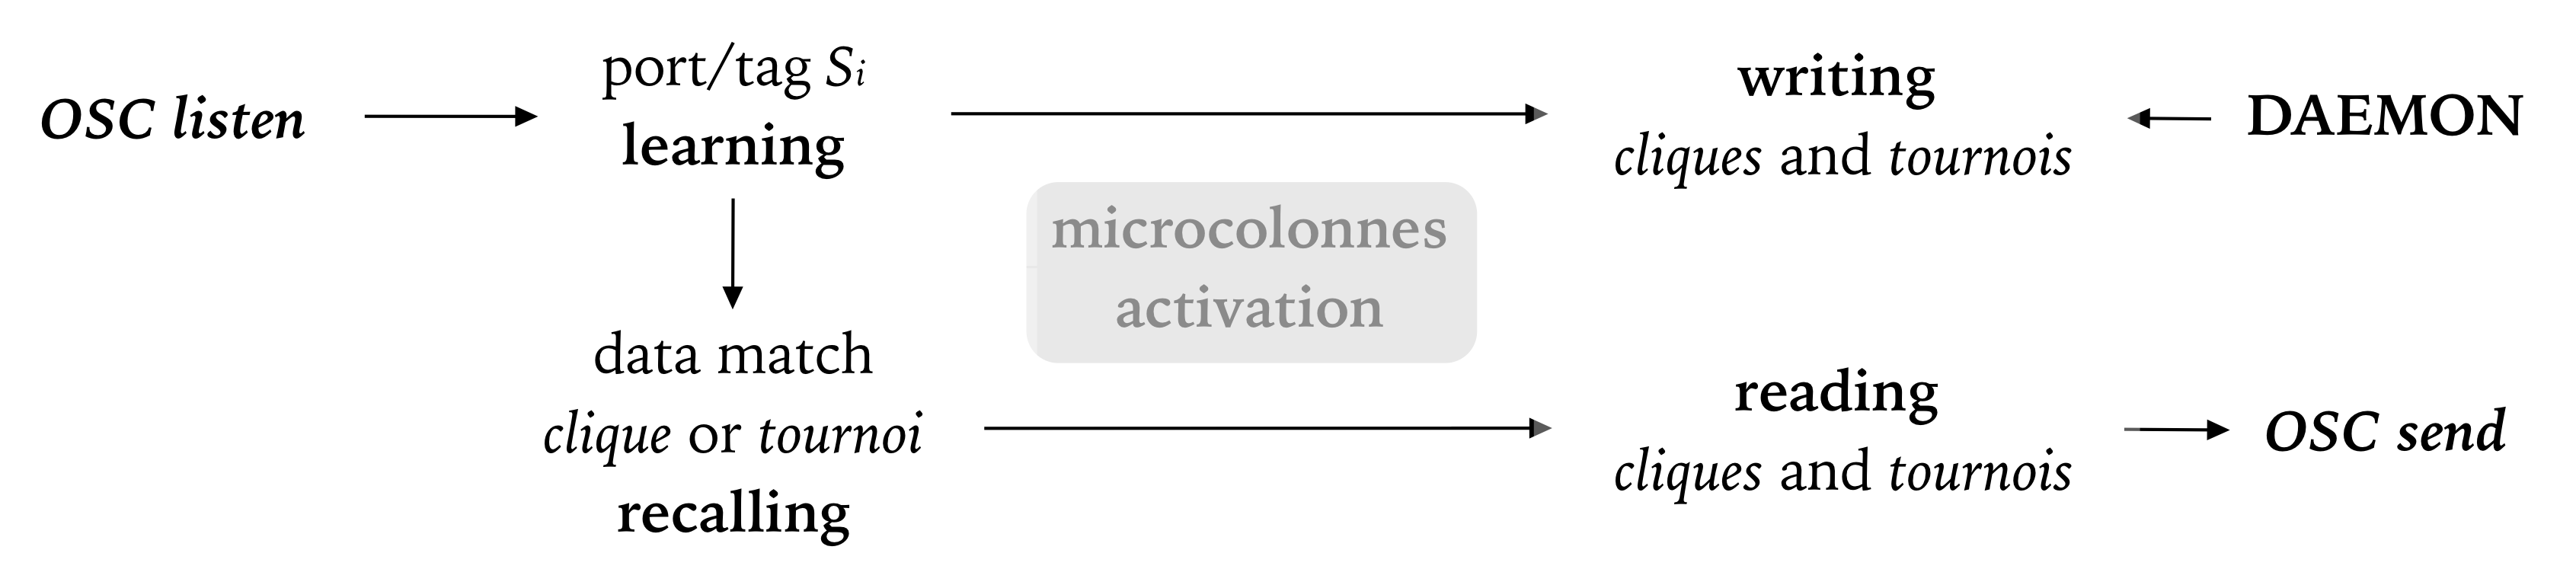
\includegraphics[width=\columnwidth]{2301}
\caption{Synoptic diagram of the I/O management. 
}
\label{fig:io}
\end{center}
\end{figure}

The AREA network can also be interpreted as it is with its inner connectionist structure.
\bigskip
\bigskip

\begin{lstlisting}[language=sectitle]
N3> (format t "~A" *CHAPTER-2*)
SELF ORGANIZING MAP
NIL
N3> 
\end{lstlisting}
\addcontentsline{toc}{section}{2. Self Organizing Map}

\bigskip
The classes SOM, RNA et NEURON are a minimalist adaptation of the code source \textsl{Neuromuse}\footnote{\href{https://github.com/FredVoisin/neuromuse}{\texttt{\scriptsize https://github.com/FredVoisin/neuromuse}}} which aims to allow a flexibility to manage parameters. In short, it is question to initiate a Self Organizing Map in terms of learning and activation. 

\bigskip

The Self Organizing Map is a concept formalised and modeled in 1980 by Teuvo Kohonen. It is a model of an artificial neural network working by competition for a set of given stimuli. This allows to create a topology for classification, interpolation or displaying multidimensional data.

\bigskip

\begin{displayquote}
The map consists of a regular grid of processing units, `neurons'. A model of some multidimensional observation, eventually a vector consisting of features, is associated with each unit. The map attempts to represent all the available observations with optimal accuracy using a restricted set of models. At the same time the models become ordered on the grid so that similar models are close to each other and dissimilar models far from each other. 

\smallskip 

Fitting of the model vectors is usually carried out by a sequential regression process, where $t = 1,2,...$ is the step index. For each sample $x(t)$, first the winner index $c$ (best match) is identified by the condition:

$$\forall i, || x(t) - m_c(t) || \leq || x(t) - m_i(t) ||$$

After that, all model vectors or a subset of them that belong to nodes centered around node $c = c(x)$ are updated as:

$$m_i(t + 1) = m_i(t) + h_{c(x),i}(x(t) - m_i(t))$$

Here $h_{c(x),i}$ is the `neighborhood function', a decreasing function of the distance between the $i$th and $c$th nodes on the map grid. This regression is usually reiterated over the available samples.\footnote{\href{http://www.cis.hut.fi/research/som-research/som.shtml}{\texttt{\scriptsize http://www.cis.hut.fi/research/som-research/som.shtml}}}
\end{displayquote}

%\bigskip
%
%First of all, here are some guidelines of how to use functions defined in the user file as parameters in N3 context. These functions require two or three arguments and optionally a list of additional argument(s). To set a function, a list is required with as first argument the function itself, and optionally the remaining option(s) belonging to the function. 

\bigskip

Here are some guidelines about the available parameters in N3.

\bigskip
%\newpage
Functions required for the class SOM as slots:

\begin{itemize}
\item The map function -- slot \texttt{carte} -- to initiate the neurons of the SOM.
\item The neighborhood function -- slot \texttt{voisinage} -- which defines the type of influence that the winning neuron will have on its neighbors allowing to update the network during the learning process (usually a gaussian or a `mexican hat' function).
\item The proximity function to define the type of relationship %(always in terms of distance, although this may be different, for example in terms of standard deviation) 
between two neurons -- slot \texttt{distance-in} --  
%involving the positions or the outputs, 
or between a set of stimuli and its response -- slot \texttt{distance-out} -- when the SOM is activated in order to set and to minimalize errors for the winning neuron selection.
\end{itemize}

\bigskip

The SOM initiation is done either with the defmethod \texttt{init-som} or simply with the N3 function \glspl{create-mlt} with as arguments the name of the SOM, the number of stimuli and the number of neurons in the map.

\smallskip

The activation consists to compute for each neuron the error defined by $|| x(t) - m_i(t) ||$. 

\smallskip

Note that the data input has to be adjusted such as each component has a value between 0 and 1 in order to match the range of the output as weight values during initialisation.

\bigskip

The learning step refers to the class RNA according to the slots:

\begin{itemize}
\item \texttt{learning-rate} as the maximum correction value applied to the winning neuron;
\item \texttt{radius} as influence of the winning neuron on its neighbors. 
\end{itemize}

\begin{figure}[htbp]
\begin{center}
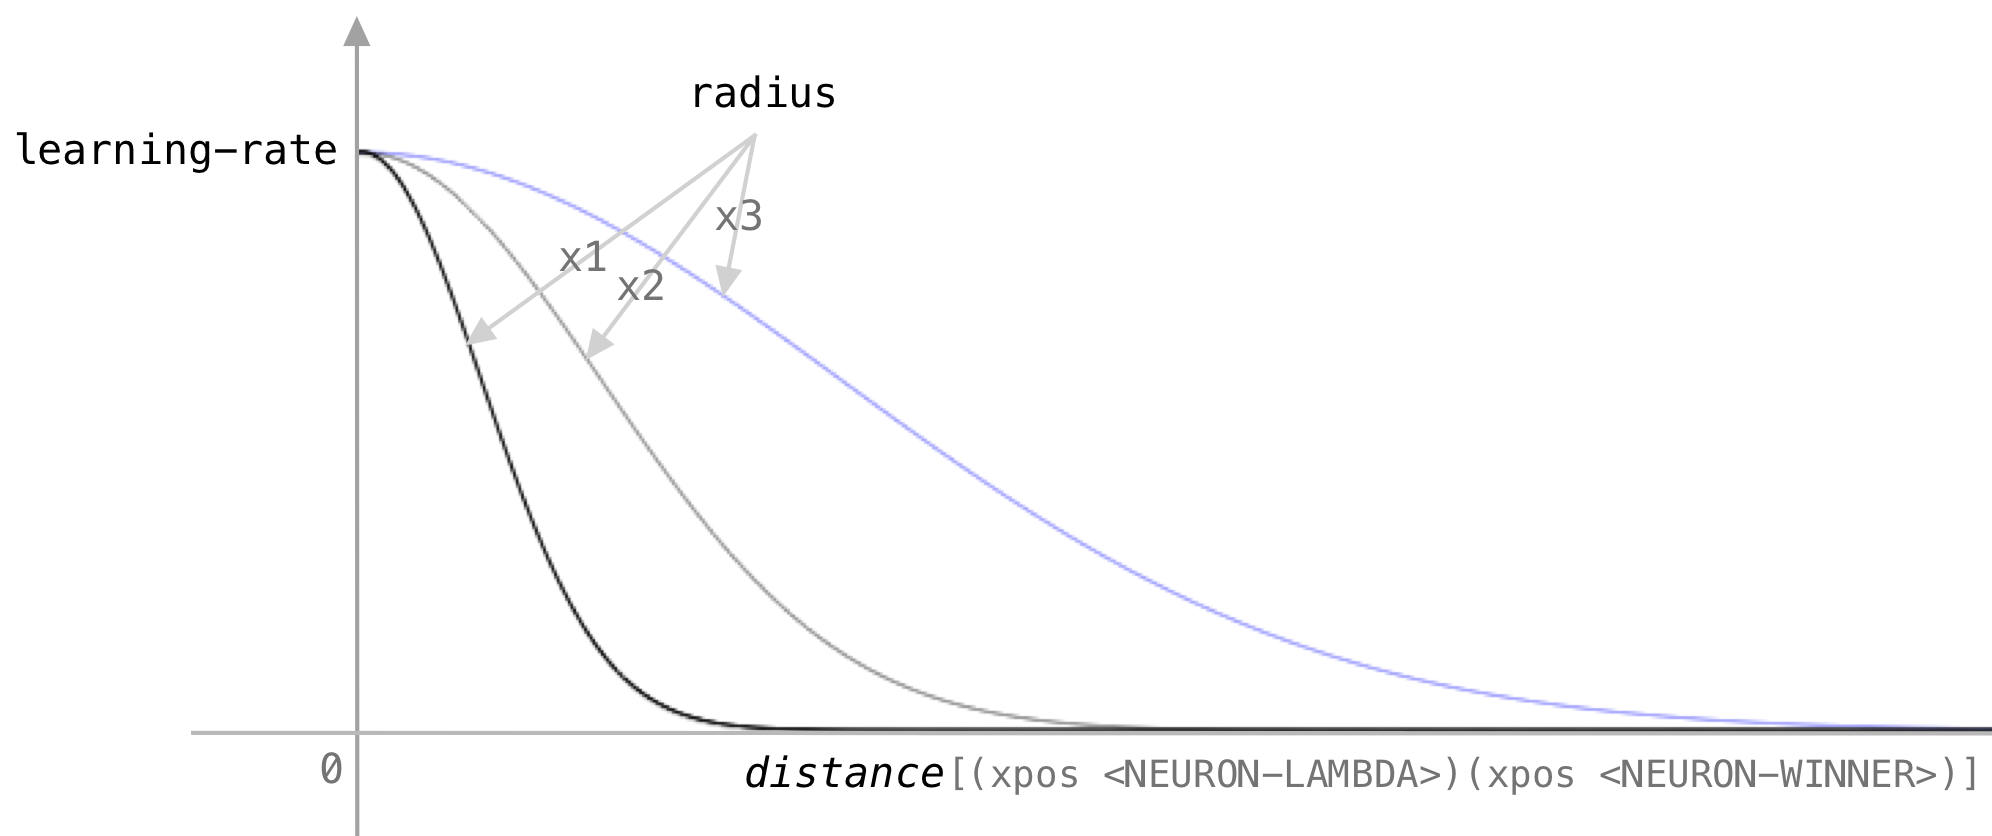
\includegraphics[width=\columnwidth]{2311}
\caption{The neighborhood function \glspl{gauss} with its parameters. %The `half' Bell shape is proportional to the radius ...
}
\label{fig:gs}
\end{center}
\end{figure}

See Table \ref{table:bf} concerning functions which can be set in a SOM as described previously. 

See also Table \ref{table:class} on page \pageref{table:class} for all parameters and properties.

\begin{table}[htp]
\caption{\label{table:bf}The package N3 provides some basic functions.}
\begin{center}
\begin{tabular}{| p{3cm} | p{5.5cm}}
Mapping & \glspl{quadrare}, \glspl{rnd-map} \\ 
Proximity & \glspl{euclidean} \\  
Neighborhood & \glspl{gauss}, \glspl{fn-mex} \\   
Decreasing & \glspl{exp-decay} 
\end{tabular}
\end{center}
\end{table}%
%\bigskip
%\bigskip
\newpage

\begin{lstlisting}[language=sectitle]
N3> (format t "~A" *CHAPTER-3*)
TOPOLOGY
NIL
N3> 
\end{lstlisting}
\addcontentsline{toc}{section}{3. Topology}
\label{topology}

\bigskip
To map a SOM, the main principle is to initiate a learning process with a significative dataset, using the decreasing function \glspl{exp-decay} applied on the learning rate and on the radius of neighbourhood influence in relation with the number of iteration, defined by $\alpha_{(t)} = \alpha_0 e^{(-t/T)}$ with $\alpha_0$ as the initial value and $T=n/|ln(\alpha_n/\alpha_0)|$ with $n$ as the number of iterations. 

\bigskip

See code on the Annex \ref{ann:color} on page \pageref{ann:color}.

\begin{figure}[htbp]
\begin{center}
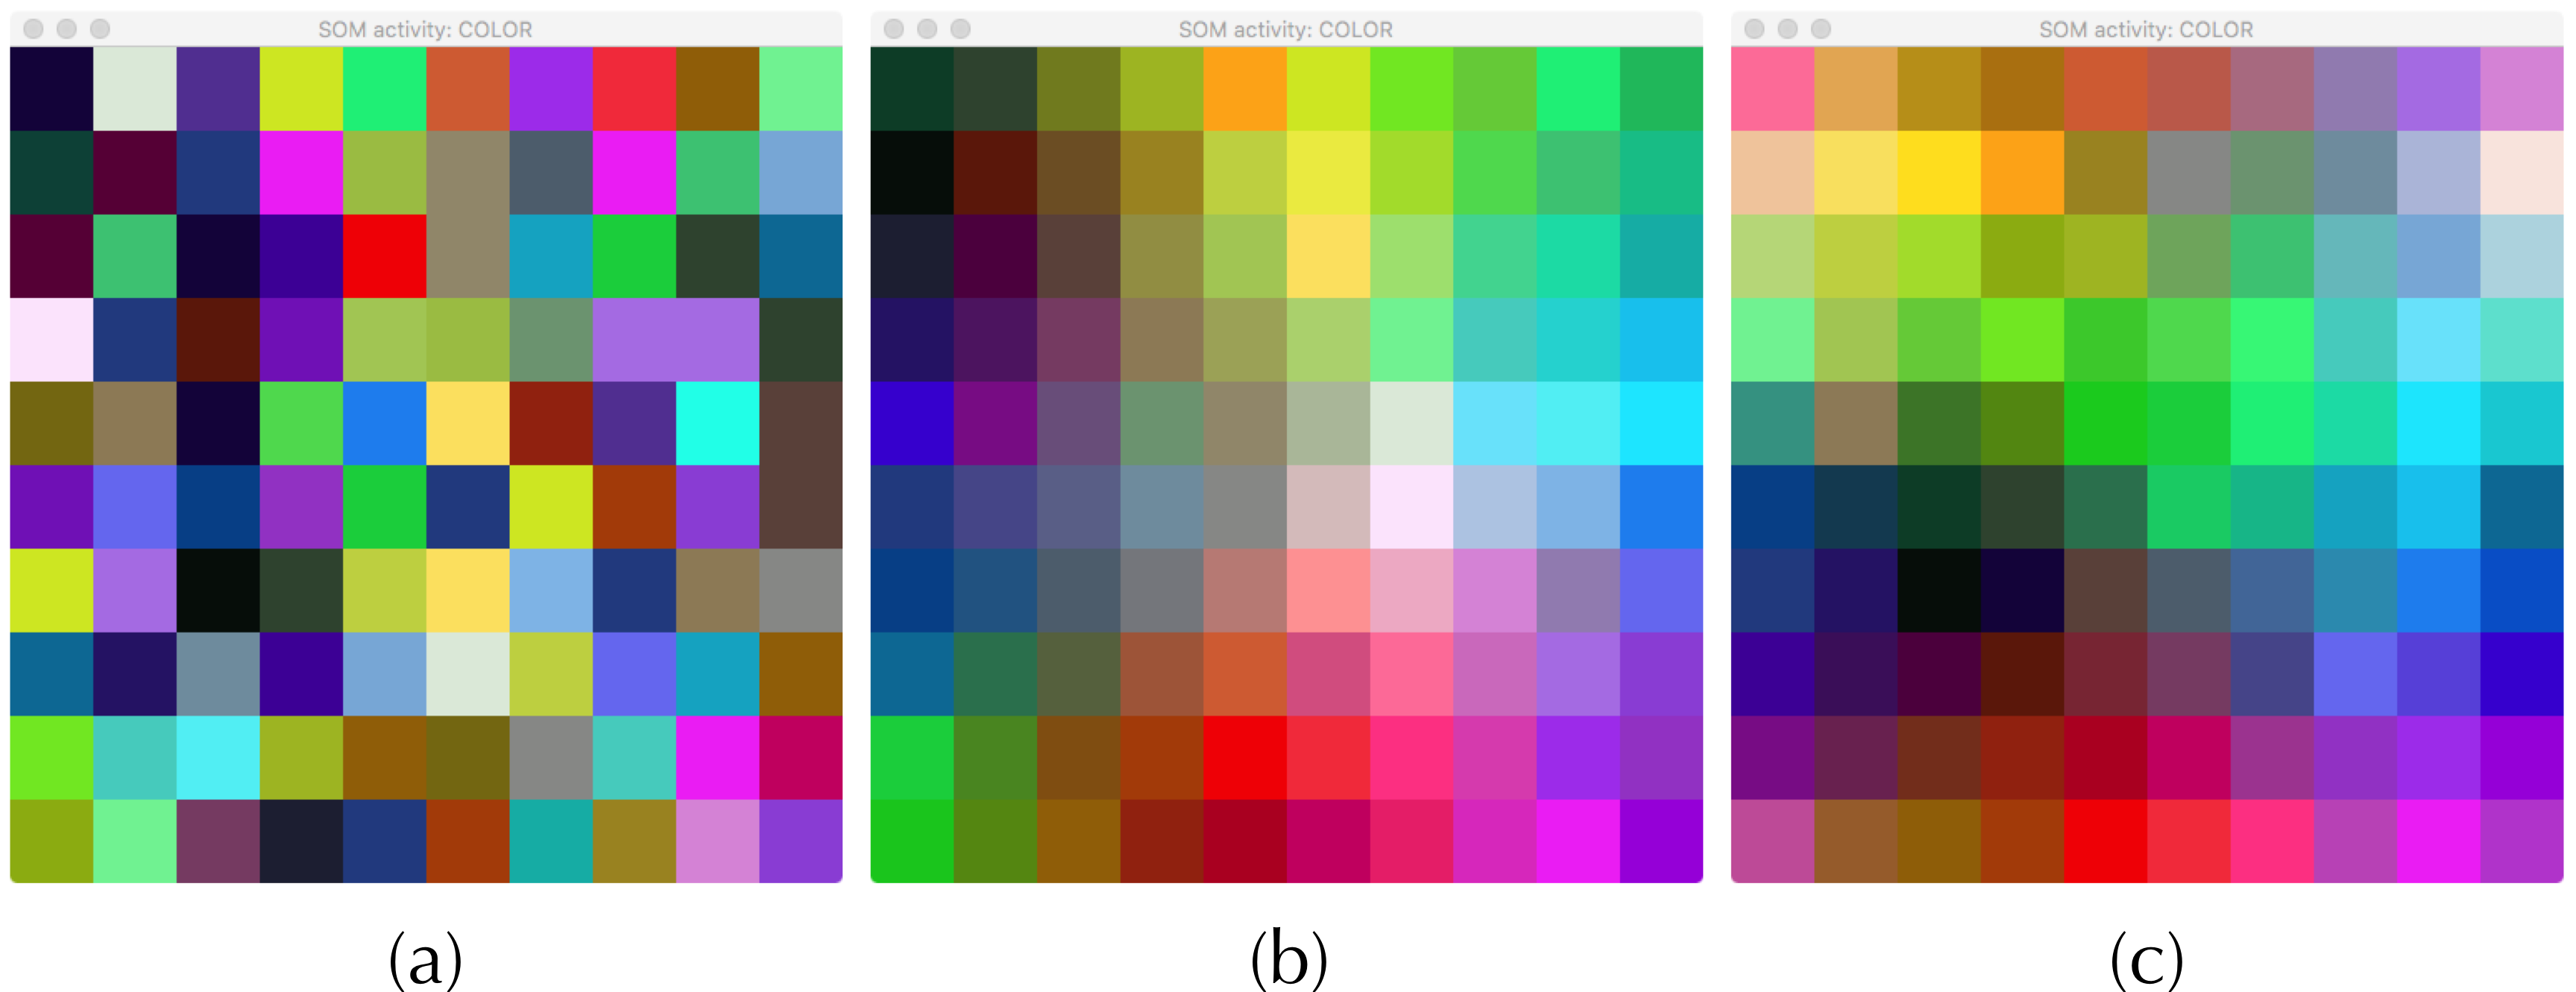
\includegraphics[width=\columnwidth]{2322}
\caption{(a) A map of 100 neurons initialised with random colors. (b) The same map after 3000 iteration. (c) Same process than (b) but with modulo.}
\label{fig:ex1}
\end{center}
\end{figure}

Note that the illustration (c) on figure \ref{fig:ex1} the modulo considers each neuron as the middle of the map. Thus, a more accurate representation of this mapping takes the form of a `donut' (i.e. a torus).
\bigskip
\bigskip

\newpage
\begin{lstlisting}[language=sectitle]
N3> (format t "~A~&;~v@{~A~:*~}~2&" *PART-2* 36 #\*)
PROLEGOMENA
;************************************

NIL
N3> (format t "~A" *CHAPTER-4*)
HIERACHICAL CLUSTERING
NIL
N3> 
\end{lstlisting}
\addcontentsline{toc}{part}{Prolegomena}
\phantomsection
\addcontentsline{toc}{section}{4. Hierarchical clustering}

\bigskip
In the framework of N3, the discrimination of the SOM in \textit{fanaux} can be carried out by hierarchical ascending classification -- noted CAH -- according to the Ward's method. The choice of the method remains empirical, but this appears the most appropriate within the framework of an automatic classification.

\bigskip

Here are some lineaments of the CAH and the Ward's method, which are described more precisely in the articles \textit{The automatic classification of quantitative data} \citep{mc} and \textit{Distances between Clustering, Hierarchical Clustering} \citep{cs}.

\begin{figure}[htbp]
\begin{center}
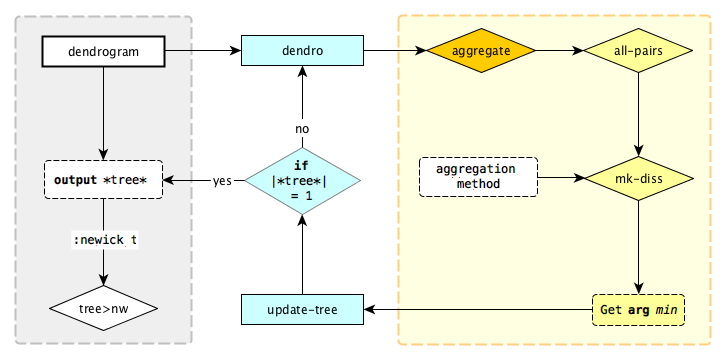
\includegraphics[width=\columnwidth]{2341}
\caption{Diagram of the CAH algorithm of \glspl{dendrogram}.}
\label{fig:cah}
\end{center}
\end{figure}

Note that \glspl{dendrogram} generates a newick\footnote{To know more about the Newick tree format see the Web page description by Joseph Felsenstein and by Gary Olsen at:\\ \indent \href{http://evolution.genetics.washington.edu/phylip/newicktree.html}{\texttt{\scriptsize http://evolution.genetics.washington.edu/phylip/newicktree.html}}} file by default allowing to display or else the tree with a third-party application.

\bigskip
\bigskip

\noindent {\large \textbf{Ward's method}}

\bigskip

With the Ward's method, the distance between two classes $A$ and $B$ is computed as follow:

$$d(A,B)=\frac{|A||B|}{|A|+|B|}d(g_{A}, g_{B})^2$$

with the mean value:

$$g_{\mathcal{P}}=\frac{1}{|\mathcal{P}|}\sum_{i \in \mathcal{P}}s_i=\overline{x}$$


In some case, the dendrogram hierarchy may have inversions. This can be avoided by applying the following relation: 

$$\forall A, B \in H, h (A \cup B) = max (d (A, B), h (A), h (B))$$

\bigskip

Finally, the intraclass inertia is computed for each node as a potential class $C$ such that:

$$I_C=\frac{1}{|C|}\sum_{e \in C}d(e,g_C)^2$$
\bigskip
\bigskip

%\newpage
\begin{lstlisting}[language=sectitle]
N3> (format t "~A" *CHAPTER-5*)
CLIQUE
NIL
N3> 
\end{lstlisting}
\addcontentsline{toc}{section}{5. Clique}

\bigskip
In graph theory, the clique -- also called complete graph -- is a set of nodes such that each node is adjacent to all others. This is expressed in the present context by a set called \textit{macrocolonne} consisting of neurons or group of neurons called \textit{microcolonne} interconnected according to the type of information concerned -- see figures \ref{fig:cli}(a), \ref{fig:cli}(b) and \ref{fig:cli}(c).

\begin{figure}[htbp]
\begin{center}
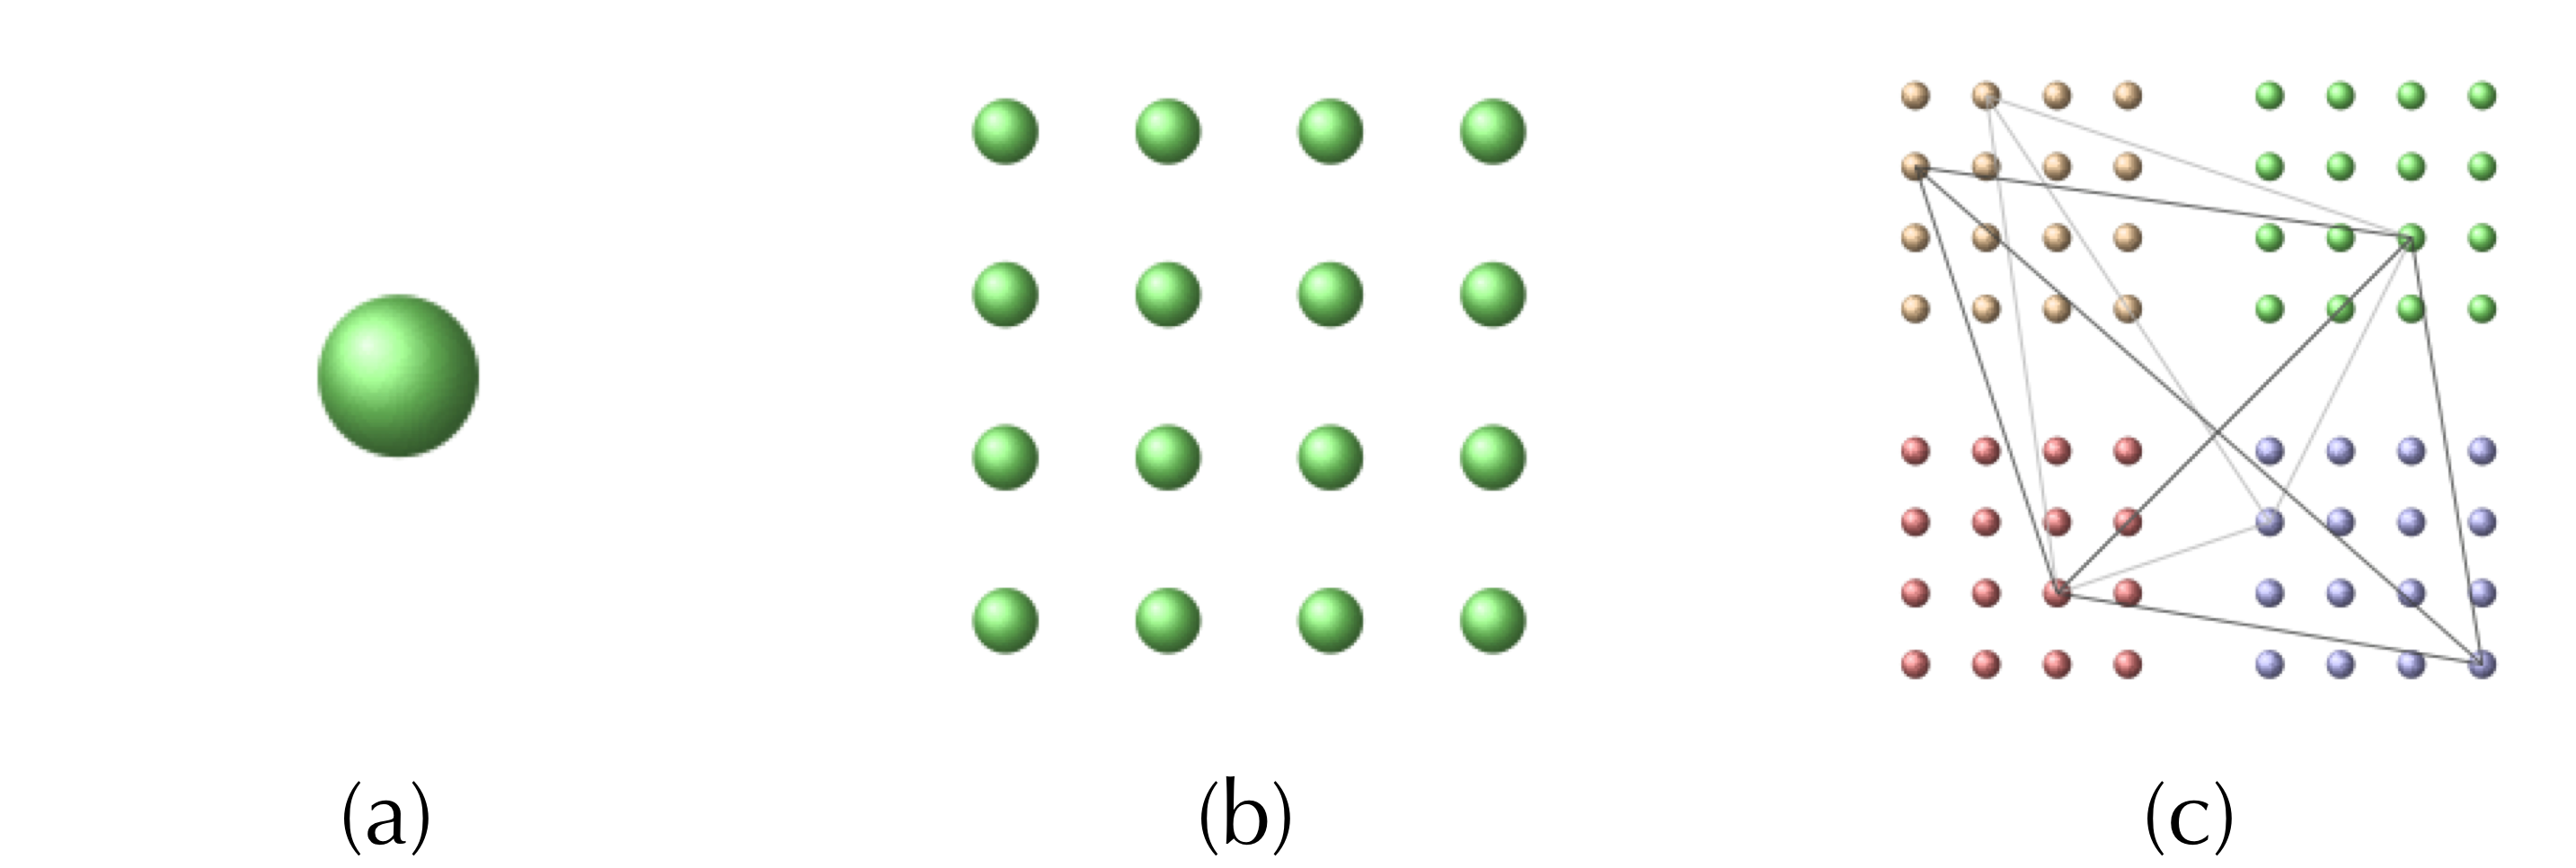
\includegraphics[width=\columnwidth]{2501}
\caption{(a) \textit{Microcolonne}: neuron or group of neurons carrying information in terms of activation potential -- e.g. a pitch of a sound. (b) \textit{Colonne}: region of \textit{microcolonnes} carrying the same type of information -- e.g. a set of pitches as a scale or other. (c) \textit{Macrocolonne}: a region of \textit{colonnes} able to carry `complete' information called `\textit{infon}' as a clique -- e.g. the characteristics of a sound defined by its pitch, intensity, duration and timbre.}
\label{fig:cli}
\end{center}
\end{figure}

On the figure \ref{fig:cli}(c), we can observe two cliques, one of which is dark gray overlays partially on the second in light gray.

\bigskip

From now on, we name indifferently as synonym \textit{microcolonnes} as \textit{fanaux} (i.e. a list of NEURON),  \textit{colonne} as MLT, \textit{macrocolonne} as AREA and \textit{infon} as a clique at the AREA level.
\bigskip
\bigskip

\begin{lstlisting}[language=sectitle]
N3> (format t "~A" *CHAPTER-6*)
TOURNOI
NIL
N3> 
\end{lstlisting}
\addcontentsline{toc}{section}{6. \textit{Tournoi}}

\bigskip
In graph theory, the \textit{tournoi} is an oriented clique. This currently inscribes a sequence in a temporal configuration, where the \textit{fanaux} -- by nature timeless -- will then create links oriented in the form of cliques, in other words \textit{tournoi}.

\begin{figure}[htbp]
    \centering
    \begin{minipage}{0.5\textwidth}
        \centering
                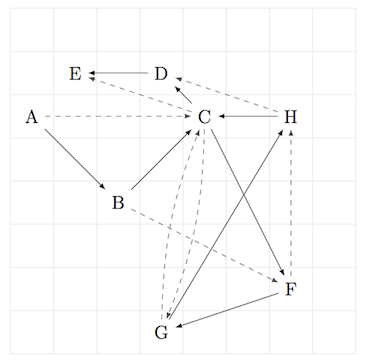
\includegraphics[width=0.9\textwidth]{2402} % second figure itself
        \caption{Example of application of \textit{tournois} \citep{bg1}, op. cit., page 117.}
        \label{fig:trn2}
            \end{minipage}\hfill
    \begin{minipage}{0.45\textwidth}
        \centering
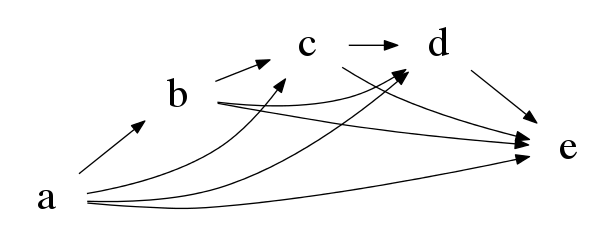
\includegraphics[width=0.9\textwidth]{2401} % first figure itself
        \caption{Here is an example of a 5 order \textit{tournoi}. This one corresponds to the followings arcs: ((a b) (a c) (a d) (a e) (b c) (b d) (b e) (c d) (c e) (d e)) and which will be translated simply by: (a b c d e).}
      \label{fig:trn1}

    \end{minipage}
\end{figure}

\bigskip

To illustrate an application of \textit{tournois}, the figure \ref{fig:trn2} shows a directed graph, in which we seek to restore the path A-B-C-F-G-H-C-D-E unambiguously -- represented with full arrows. Each node symbolizes an \textit{infon}. At first, the problem lies at node C, where two options are possible, namely F or D. A \textit{tournoi} of order 3 solves this problem, covering 2 successive nodes -- represented by dashed arrows --, anticipating thus the path from C to F signaled by the arrows from B to F when we come from B.

\bigskip

Thus, the temporal overlap depends on the order\footnote{In the graph theory, the order is the number of nodes interconnected. For both the \textit{tournoi} and the clique as a complete graph, the order allows to determinate the number of edges needed such as for a graph of order $n$, the number of edges is equal to $n(n-1)/2$ -- see example figure \ref{fig:trn1}.} of the \textit{tournoi}, i.e. $n-1$ and will determine the anticipation capacity of the network.
\bigskip
\bigskip

\begin{table}
\small
\centering
\begin{tabular}{r*1{c>{\ttfamily}l}cll}
  
  &   & \normal{\head{Slot}} & \normal{\head{\hspace{2mm} Input}}
  & \normal{\head{Note}} \\
  
    \midrule
 
  \multirow{7}{*}{NEURON} 
  &   & name & NEURON &  \\
  &   & net & RNA &   \\
  &   & xpos & \itshape list & as coordinates  \\
  &   & synapses-list & \itshape list  &   \\
  & \faCog  & temperature & \itshape number &   \\
  &   & erreur & \itshape number &   \\
  &   & output & \itshape list &   \\
  
    \midrule

\multirow{12}{*}{RNA} 
  &  \begin{minipage}{.023\textwidth}
\includegraphics[width=\linewidth]{1124}\end{minipage} & name & SOM &  \\
  &  \begin{minipage}{.023\textwidth}
\includegraphics[width=\linewidth]{1124}\end{minipage} & nbre-neurons & \itshape integer &   \\
  &   & neurons-list & \itshape list &   \\
  & \begin{minipage}{.023\textwidth}
\includegraphics[width=\linewidth]{1124}\end{minipage}  & nbre-input & \itshape integer &   \\
  & \faCog  & input & \itshape list &  \\
  &  \faCog & radius & \itshape number &   \\
  &  \faCog & learning-rate & \itshape number &   \\
  &   & date-report & \itshape hash-table  &  \\
  &   & epoch & \itshape integer &   \\
  &  \begin{minipage}{.025\textwidth}
\includegraphics[width=\linewidth]{1123}\end{minipage} & udp-list & \itshape list &   \\
  &  \begin{minipage}{.025\textwidth}
\includegraphics[width=\linewidth]{1123}\end{minipage} & daemons & \textit{thread}$|$\textit{list} &  \\
  &  \begin{minipage}{.025\textwidth}
\includegraphics[width=\linewidth]{1123}\end{minipage} & superdaemon & \textit{thread}$|$\textit{list} &   \\
  
  \midrule

 \multirow{7}{*}{SOM} 
  &   & neuron-gagnant & NEURON &  \\
  &  \faCog & distance-in & \itshape function &   \\
  &  \faCog & distance-out & \itshape function &   \\
  &  \faCog & voisinage & \itshape function &   \\
  & \begin{minipage}{.023\textwidth}
\includegraphics[width=\linewidth]{1124}\end{minipage}  & carte & \itshape function &  \\
  &  \begin{minipage}{.023\textwidth}
\includegraphics[width=\linewidth]{1124}\end{minipage} & field & \textit{number}$|$\textit{list} &  {\footnotesize if \textit{list}; $||$\texttt{field}$||$ = \texttt{topology}} \\
  &  \begin{minipage}{.023\textwidth}
\includegraphics[width=\linewidth]{1124}\end{minipage} & topology & \itshape integer &   \\
  
  \midrule
  
   \multirow{6}{*}{MLT} 
  &   & net & AREA &  \\
  &  \faCode & fanaux-list & \itshape list & $\rightarrow$ \glspl{update-fanaux} \\
  & \faCode  & cover-value & \itshape integer & $\rightarrow$ \glspl{update-cover-value} \\
  &   & mct & \itshape list &   \\
  &   & onset & \itshape hash-table &   \\
  &   & fine & \itshape hash-table &   \\
  &   & trns & \itshape hash-table &   \\
  &   & arcs & \itshape hash-table &   \\
  
  \midrule
  
   \multirow{8}{*}{AREA} 
  &  \begin{minipage}{.023\textwidth}
\includegraphics[width=\linewidth]{1124}\end{minipage} & name & AREA &  \\
  &  \begin{minipage}{.023\textwidth}
\includegraphics[width=\linewidth]{1124}\end{minipage} & soms-list & \itshape list &   \\
  &   & fanaux-length & \itshape integer &   \\
  &   & current-clique & \itshape list &   \\
  & \faCog  & sensorial-rate & \itshape number &   \\
  &   & arcs & \itshape hash-table &   \\
  &   & date-report & \itshape hash-table &  \\
  & \begin{minipage}{.025\textwidth}
\includegraphics[width=\linewidth]{1123}\end{minipage}  & udp-list & \itshape list &   \\
  
\end{tabular}
\caption{\label{table:class}List of N3 classes with their respective slots.}
\end{table}

\begin{lstlisting}[language=sectitle]
N3> (format t "~A~&;~v@{~A~:*~}~&" *PART-3* 36 #\*)
SHORT-TERM MEMORY
;************************************
NIL
N3> 
\end{lstlisting}
\addcontentsline{toc}{part}{Short-term memory}

\bigskip
For a given sequence as a learning process, the \textit{tournois} are indexed for each \textit{colonne} at the level of the class MLT, whose order will be defined by the slot \texttt{cover-value}. The \textit{tournois} (with \texttt{remanence}\footnote{The remanence means if we consider the \textit{tournois} with the cover-value as they are recorded (i.e. the order of the \textit{tournois}) or if we only consider the arcs.} \textit{true}) and the arcs constituting the \textit{tournois} (with \texttt{remanence} \textit{nil}) will be retained in a separate hash table associated with each SOM.

Note that \texttt{cover-value} must imperatively be an integer and greater than or equal to 3 (since a \textit{tournoi} is defined only from 3 nodes).

\bigskip

The \textit{microcolonnes} of each SOM are listed and indexed according to their symbolic representation -- i.e. the type of information conveyed, triggered by \textit{stimuli} -- in the slot \texttt{fanaux-list} as a list of neurons. In other words, the 
\textit{microcolonnes} is the SOM reduced to the fanaux-list.
\bigskip

\begin{lstlisting}[language=N3]
(update-fanaux SOMNAME <int>) ; if needed
(dolist (k SEQUENCCE)
  (setf (input SOMNAME) k)
  (learn SOMNAME :seq t))
\end{lstlisting}

\bigskip

N3 allows if needed to update by surjection\footnote{The surjection algorithm consists to explore the distance matrix of the `new-fanaux-list' from `the old-fanaux-list' in order to retain only the neurons with the smallest distance per row and by column. The conjunction of the last two is listed according to the index of the `old-fanaux-list', adding if necessary the intermediate distances.\label{surj}} the fanaux-list with the method \glspl{update-fanaux} according to the `old-fanaux-list' -- if this latest is not nil. This means the modification of the arcs (at the SOM level) and of the involved edges (at the AREA level) if applicable. Mind that this will inevitably lead to an alteration -- more or less significant depending on the degree of change -- of what has been learned so far.

\bigskip
There are two ways to read the acquis of the MLT. The first one consists to retrace one (or more) \textit{tournoi(s)} from a partial sequence temporally ordered according to the remanence or not. The method \glspl{locate-tournoi} allows to do that and gives as result a list of potential \textit{tournoi(s)} sorted according to their weight. 

\bigskip
\begin{lstlisting}[language=N3]
(locate-tournoi SOMNAME '(3 ? 0) :remanence nil)
; ((0.28400004 (3 2 0)) (0.22000018 (3 3 0)) (0.2 (3 0 0)) (0.15999967 (3 1 0)) (0.13600005 (3 4 0)))
(locate-tournoi SOMNAME '(3 ? 0) :remanence t)
; ((0.5 (3 2 0)) (0.5 (3 3 0)))
\end{lstlisting}
\bigskip

Note that with the remanence case, the given \textit{tournoi} is compared with the learned \textit{tournois} of MLT, and each match is retained with its weight, then the sum of all these weights is normalised. In the case of the length of the given \textit{tournoi} is superior to the \texttt{cover-value}, this one is decomposed as follow: for instance consider the tournoi \texttt{(a b c d e)} and the \texttt{cover-value} equal to 3, then the computation is done on \texttt{(a b c) (b c d)} and  \texttt{(c d e)}.

\smallskip

Also, to limit the search space -- which increases exponentially -- each \textit{tournoi} composed with only wild cards is avoided. In that case, there are two undocumented functions to do the job as \texttt{all-tournoi} -- which lists all the possible \textit{tournois} according to a given order and the remanence as keys -- and \texttt{rnd-tournoi} -- which chooses randomly but weighted from the previous result.

\bigskip

The second one expresses the previous result in terms of probability by `postpended' a wild card. 
Thus, the method \glspl{next-event-probability} allows to compute the probability of occurrences for a \textit{fanal} to occur after a given subsequence of \textit{fanaux} -- as a list of indexed \textit{fanaux} temporally ordered (with the possibility to add `?' as a wild card).

\smallskip

Then, the purpose of this function allows to estimate an occurrence -- with the key \texttt{:result :eval} (set by default) -- through the key function \texttt{:compute} (set with the function \texttt{rnd-weighted} by default). 

The function \texttt{rnd-weighted} allows to choose a number at random between $0$ and $1$ such as this interval is conformed to the ordered repartition of probabilities (see the coloured stripes on figure \ref{fig:colstr} corresponding to the following code snippets).

%\vspace{-5mm}
\smallskip

\begin{lstlisting}[language=N3]
(next-event-probability '(3 ? 0) SOMNAME :remanence nil     :result :verbose) 
; 2 => 30.749 %
; 3 => 22.460 %
; 0 => 16.756 %
; 1 => 16.043 %
; 4 => 13.993 %
\end{lstlisting}

%\bigskip
%\newpage

\begin{lstlisting}[language=N3]
(next-event-probability '(3 ? 0) SOMNAME :remanence t       :result :verbose) 
; 0 => 28.571 %
; 2 => 23.810 %
; 1 => 19.048 %
; 3 => 19.048 %
; 4 =>  9.524 %
\end{lstlisting}

\begin{figure}[htbp]
\begin{center}
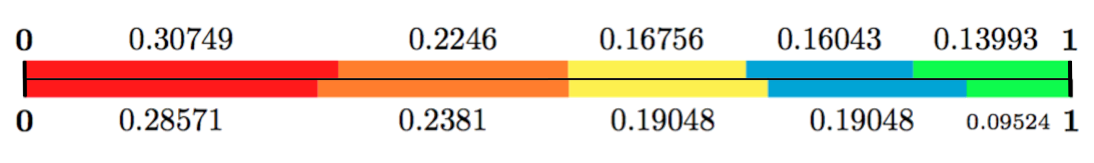
\includegraphics[width=\columnwidth]{1301}
\caption{Coloured stripes of the distributed probabilities without remanence on the top and with remanence at the bottom.}
\label{fig:colstr}
\end{center}
\end{figure}




\bigskip
\bigskip

\begin{lstlisting}[language=sectitle]
N3> (format t "~A~&;~v@{~A~:*~}~&" *PART-4* 36 #\*)
LONG-TERM MEMORY
;************************************
NIL
N3> 
\end{lstlisting}
\addcontentsline{toc}{part}{Long-term memory}

\bigskip
This is one of the main part of \textsl{Neuromuse3}. Indeed, the aim here is to create connections between each \textit{microcolonne} -- or \textit{fanal} -- as \textit{tournois} inside a neuronal AREA as cliques. 

Then, the learning process consists to connect a set of SOM together in order to create an associative memory.

\bigskip

The \textit{macrocolonne} is managed by the class AREA, establishing the connections of each clique from each identified \textit{fanal} involving relationships with incoming and outgoing arcs for each \textit{fanal}. Then, each arc as the key of the hash table of AREA will be associated to a weight.

%add here example or clarity

\bigskip

As seen previously, the method  \glspl{locate-tournoi} gives as result a list of potential  \textit{tournois}, which by cross-checking with the \textit{tournois} of the other \textit{colonnes} -- correlated  in terms of cliques -- allow the (re-)construction\footnote{The (re-)construction must be understood in terms of reminder and invention.} of a sequence according to the user `condition(s)'. 

\smallskip

In the same vein, the method \glspl{locate-clique} allows to retrace clique(s) from partial data. Thus, from this step, the (re-)construction of a sequence which is connected to the reading of \textit{tournois}, is done in a field of arcs and edges according to a deliberate heuristic by consensus and iteration.

\smallskip

The (re-)construction is effective when a learned sequence can be retraced as recollection or retrieving memory or as creation. In all case, this implies modalities defined by the user -- see diagram on figure \ref{fig:mlt2}\footnote{Concerning the diagram of the figure \ref{fig:mlt2}:
\begin{itemize}
\item[$\bullet$]  The constraints or rules allow to limite the field of search, or in other words the constraints aims to reduce the field of possibilities. This can be done with as examples, harmonic rules, a specific scale or whatever. It would be possible to define the `rules' on an interactive way, as a live coding for instance -- involving  in both case the user with its own code --, allowing the adaptability in terms of reaction to the immediate environment.
\item[$\bullet$]  The bayesian inference can play a role for the estimation of a response in terms of probability focusing on the acquis -- that is to say the highest probability.
\item[$\bullet$]  The resolution is done on the filtered probabilities in order to get an optimal solution, which one can be oriented with some a posteriori rule(s) of the user. 
\item[$\bullet$] Note that for now, the user interaction allows to manage the interrelationship between the agent and its environment in terms of affect.
\end{itemize}}.

\bigskip

\begin{figure}[htbp]
\begin{center}
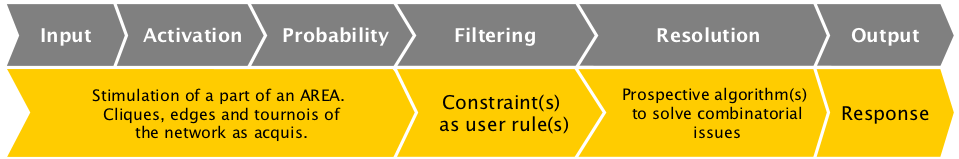
\includegraphics[width=\textwidth]{2551}
\caption{Synoptic diagram of resolution I/O at the AREA level.}
\label{fig:mlt2}
\end{center}
\end{figure}

%\item[$\bullet$]  The valence of a potential response fits within context of  predictability.

%\bigskip
%\newpage
The method \glspl{locate-clique} allows a first estimation of possible clique(s) according to two possible inputs:
\begin{enumerate}
\item isolated node(s): \texttt{((microcolonne\_indice colonne\_indice) …)}
\item ordered node(s): list of \textit{microcolonne} indice(s) and/or wild card ordered according to the soms-list. \label{txt:on}
\end{enumerate}

All connected  \textit{microcolonnes} to known elements are listed. This is what we observe on the figure \ref{fig:mlt1} with the nodes (4 0) and (1 3), respectively the fifth \textit{fanal} of SOM 1 and the second \textit{fanal} of SOM 4. 
All microcolonnes whose connection number is equal to the number of known elements are collected. These connections are represented in solid lines.

\smallskip

Thus, we obtain a list of potential cliques ordered according to their respective weights in terms of probability. 

%\newpage
\begin{figure}[h]
\begin{center}
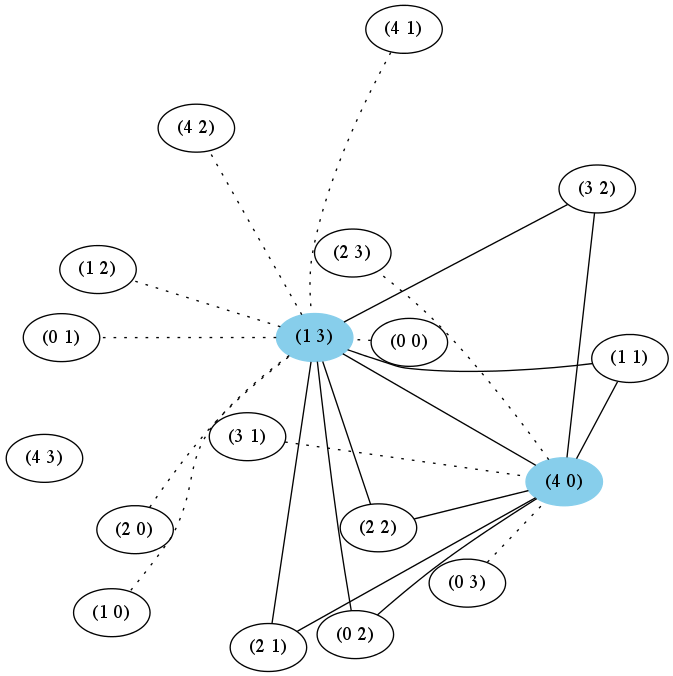
\includegraphics[width=9cm]{2701}
\caption[Cliques estimation on a network AREA (partial view) composed of four SOM of five \textit{fanaux}.]{Cliques estimation on a network AREA (partial view\protect\footnotemark) composed of four SOM of five \textit{fanaux}.}
\label{fig:mlt1}
\end{center}
\end{figure}

\footnotetext{Generated with \color{n3comment}{{\small \texttt{(N3::>dot AREANAME \textquotesingle((4 0) (1 3)))}}}.}

\begin{lstlisting}[language=N3]
(locate-clique AREANAME '((4 0) (1 3))) ;; isolated nodes
;; or 
(locate-clique AREANAME '(4 ? ? 1)) ;; ordered nodes
; ((0.25050917 (4 2 2 1)) (0.22403261 (4 2 3 1))  
;  (0.1965377 (4 2 0 1)) (0.120162934 (4 1 2 1))
;  (0.104887985 (4 1 3 1)) (0.10386966 (4 1 0 1)))
\end{lstlisting}
%whose indexation is modeled on the soms-list. Then, following the example of figure \ref{fig:mlt1}, we obtain: (4 (2 1) (2 3 0) 1). The elements of this list are the possible clique(s) from the proposed edges, which are listed in order to be ordered according to the weights of their links.

\bigskip

As seen before in the part 3 \textsl{Short-Term Memory}, it is possible at the AREA level to compute a potential clique according to some previous -- can be partial -- cliques interpreted in time as \textit{tournois} with or without remanence with the function \glspl{next-event-probability}. The latter takes as the \textit{head} argument a list of temporally ordered clique(s) and these are a list of ordered nodes in accordance with the second point seen previously on page \pageref{txt:on} referring to \texttt{locate-clique}.

\smallskip

To estimate the weight of a potential clique -- as for the \textit{tournoi} (except with remanence) -- one takes the mean value of the weights of all edges constituting such clique or \textit{tournoi}. 

\smallskip
%\newpage
Concerning the remanence at the AREA level, the probability for a given clique is done according to the previous cliques in terms of \textit{tournois} (also with remanence) as:

$$P_{C(T)} = \displaystyle \prod_{i \in SL} P(E_{n_i}|E_{p_i})$$

With $SL$ as the \texttt{soms-list}, $E_{n}$ as the next event -- in other words the next clique or `\textit{infon}' -- and  $E_{p}$ as the previous events.

\smallskip

Otherwise, this is the probabilities in terms of normalised weighted edges.

\bigskip
\bigskip

\noindent {\large \textbf{AREA instantiation}}

\bigskip

To create an AREA, it needs first of all to set all needed SOM requisite for the `\textit{infon}'. Then, the method \glspl{create-area} connect all these SOM according to their order in the soms-list.

\bigskip

Let the following procedure be an illustration of the principle of the learning processes at the AREA level.

\begin{lstlisting}[language=N3]
;; Create AREA
(create-mlt 'SOMNAME1 116 100 :carte #'quadrare)
(create-mlt 'SOMNAME2 5 100 :carte #'quadrare )
   ...
(create-area 'AREANAME (list SOMNAME1 SOMNAME2 ...))

;; Mapping 
(loop
   for i in '(SOMNAME1 SOMNAME2 ...)
   for data in '("~/dat1" "~/dat2" ...)
   ;; ------------------
   ;; set SCALING key(s) as a list of key+val for each SOM
   for kv in '((keyword val ...) ...) 
   ;; ------------------
   do
   ;; if needed
   (setf (distance-in (id i))
	   (lambda* (a b) (euclidean a b :position t :modulo t)))
   ;; ------------------
   (mapping (id i) 50000 (read-data (id i) data) :ds kv))
       
;; Learn the sequence `in time'.
(learn AREANAME :seq '("~/dat1" "~/dat2" ...))
\end{lstlisting}

\bigskip
Following this procedure, mind the ordered arrangement of the sequence between the \texttt{soms-list} of the AREA and the list of data.

Note that each element of the sequence can be a path as a string or as a pathname or a data list.

\bigskip 
%\newpage
\begin{figure}[!ht]
\begin{center}
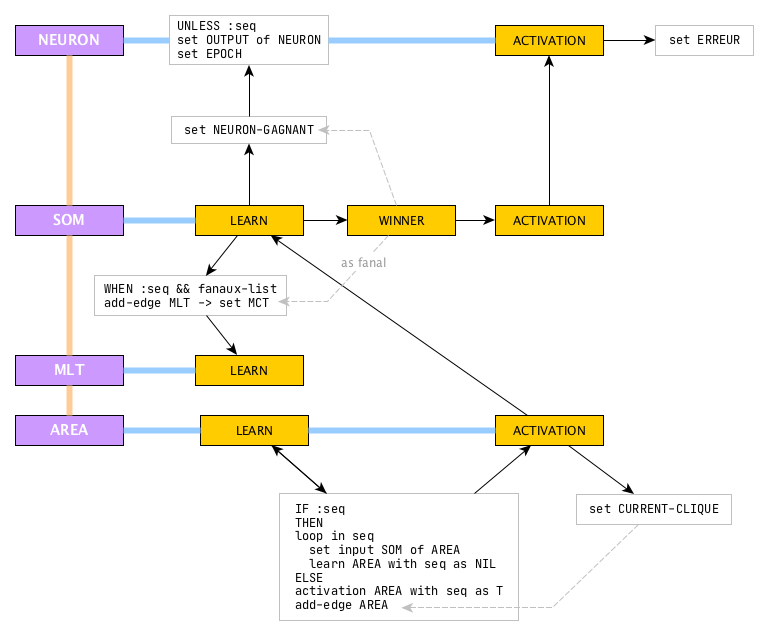
\includegraphics[width=\columnwidth]{4356}
\caption[Summary of the learning process in N3.]{Summary of the learning process in N3\protect\footnotemark.}
\label{fig:resn3}
\end{center}
\end{figure}

\footnotetext{Note that:\begin{itemize}
\item[$\bullet$] the learning is dependant of the encoding in relation to the desired environment or the kind of required `control';
\item[$\bullet$]  each sequence is identified upstream and downstream by a `\textit{tout-à-zéro}' marker; 
\item[$\bullet$]  the learning at the AREA level consists to activate the current clique (via \textit{microcolonnes} activation) in order to record it as arcs. At the same time, each MLT records arcs and \textit{tournois} connected to the previous clique. 
\end{itemize}}

\setlength{\textfloatsep}{5pt}

Before launching the learning process of the AREA, it is necessary to set the \texttt{fanaux-list} 
either \textit{a priori} with the key \texttt{n-fanaux} within the function \glspl{create-mlt} or \textit{a posteriori} with the function \glspl{update-fanaux}. In the last case, one can estimate the optimum number of \textit{fanaux} according to the user cons-traint(s) by computing the \glspl{dendrogram}. Then \texttt{(open-graph *tree*)} allows displaying the corresponding curve as the sum of the intra-class inertia by trimming with lines as peaks of the curve -- meaning the minimum distance from the parent node (as the second number in the square bracket, the first number is the number of classes at this point). Note that in the graph, the impulse segments are displayed in a logarithmic scale for better readability. At this point, the approach is rather empirical, but it should be done once and for all.

\bigskip
\bigskip

\noindent {\large \textbf{About scaling}}
\label{pt:as}

\bigskip

The bias in N3 is to normalise the input data in order to fit in a range between 0 and 1. The function \glspl{scaling} allows managing any input data according to some modalities applied at the SOM level (key \texttt{:mlt}). By default, the `data-scale' is bypassed. Then, to initiate or to interpret the data inputs, one needs to consider the following parameters:
\begin{itemize}
\item[] \myuline{\textbf{the range}} which is estimated by default between the minimal value and the maximal value of the dataset (any other values outside the range will be clipped);
\newpage

\item[] \myuline{\textbf{the curve}} allows to set the scale of the input data such as if this value equal to 0 (linear) then: 
%source: https://github.com/supercollider/supercollider/blob/develop/SCClassLibrary/Common/Math/SimpleNumber.sc
$$dataOut=\frac{(dataIn-inMin)(outMax-outMin)}{inMax-inMin}+outMin$$
and if the input data $< 0$ (concave, negatively curved as exponential scale with the value $1-e$) or $> 0$ (convex, positively curved as a logarithmic scale with the value $e-1$) then:
$$dataOut=ln\left(\dfrac{b-dataIn}{a}\right)\dfrac{outMax-outMin}{curve}+outMin$$
$$\text{with } b=inMin+a \text{ and }  a=\dfrac{inMax-inMin}{1-e^{curve}}$$ the value of the curve should be set between $+18$ and $-16$\footnote{These are some empirical limit values and, these can be different depending on the operating system and the lisp implementation.} to avoid division by zero due to some rounding caused by computer systems about floating point numbers \citep{re};
\item[] \myuline{\textbf{the type}} of the data input as:
\begin{itemize}
\item[$\bullet$] \textbf{norm} valid for all numbers, the argument is the range as a list with `minval' and `maxval' plus optionally the value of the curve (0 by default), or a number as the curve value; %if the range is known;
\item[$\bullet$] \textbf{dim} allows scaling data according to its dimension rank as a list of \textbf{norm} value by dimension.
\end{itemize}
\end{itemize}
The key \texttt{:update} set to \textit{t} records the current settings of \glspl{scaling} in the history of the SOM and will be the default scaling settings. 


\bigskip
\bigskip

\newpage
\begin{lstlisting}[language=sectitle]
N3> (format t "~A~&;~v@{~A~:*~}~&" *PART-5* 36 #\*)
DEVELOPMENTAL LEARNING
;************************************
NIL
N3> 
\end{lstlisting}
\addcontentsline{toc}{part}{Developmental learning}

\bigskip
Project launched in October 2014 by Olivier Georgeon on the internet platform MOOC\footnote{\href{http://liris.cnrs.fr/ideal/mooc/}{\texttt{\scriptsize http://liris.cnrs.fr/ideal/mooc/}}\label{noteideal}} consisting of learning and developing a new concept in artificial intelligence called IDEAL (\textbf{I}mplementation of \textbf{DE}velopment\textbf{A}l \textbf{L}earning) -- defined as an ``approach to simulate the early mechanisms of emergent cognition based on theories of enactive cognition and on constructivist epistemology'' \citep{ger}.

\begin{wrapfigure}{r}{0.35\textwidth}
\vspace{-5pt}
   \hspace{-5pt} 
   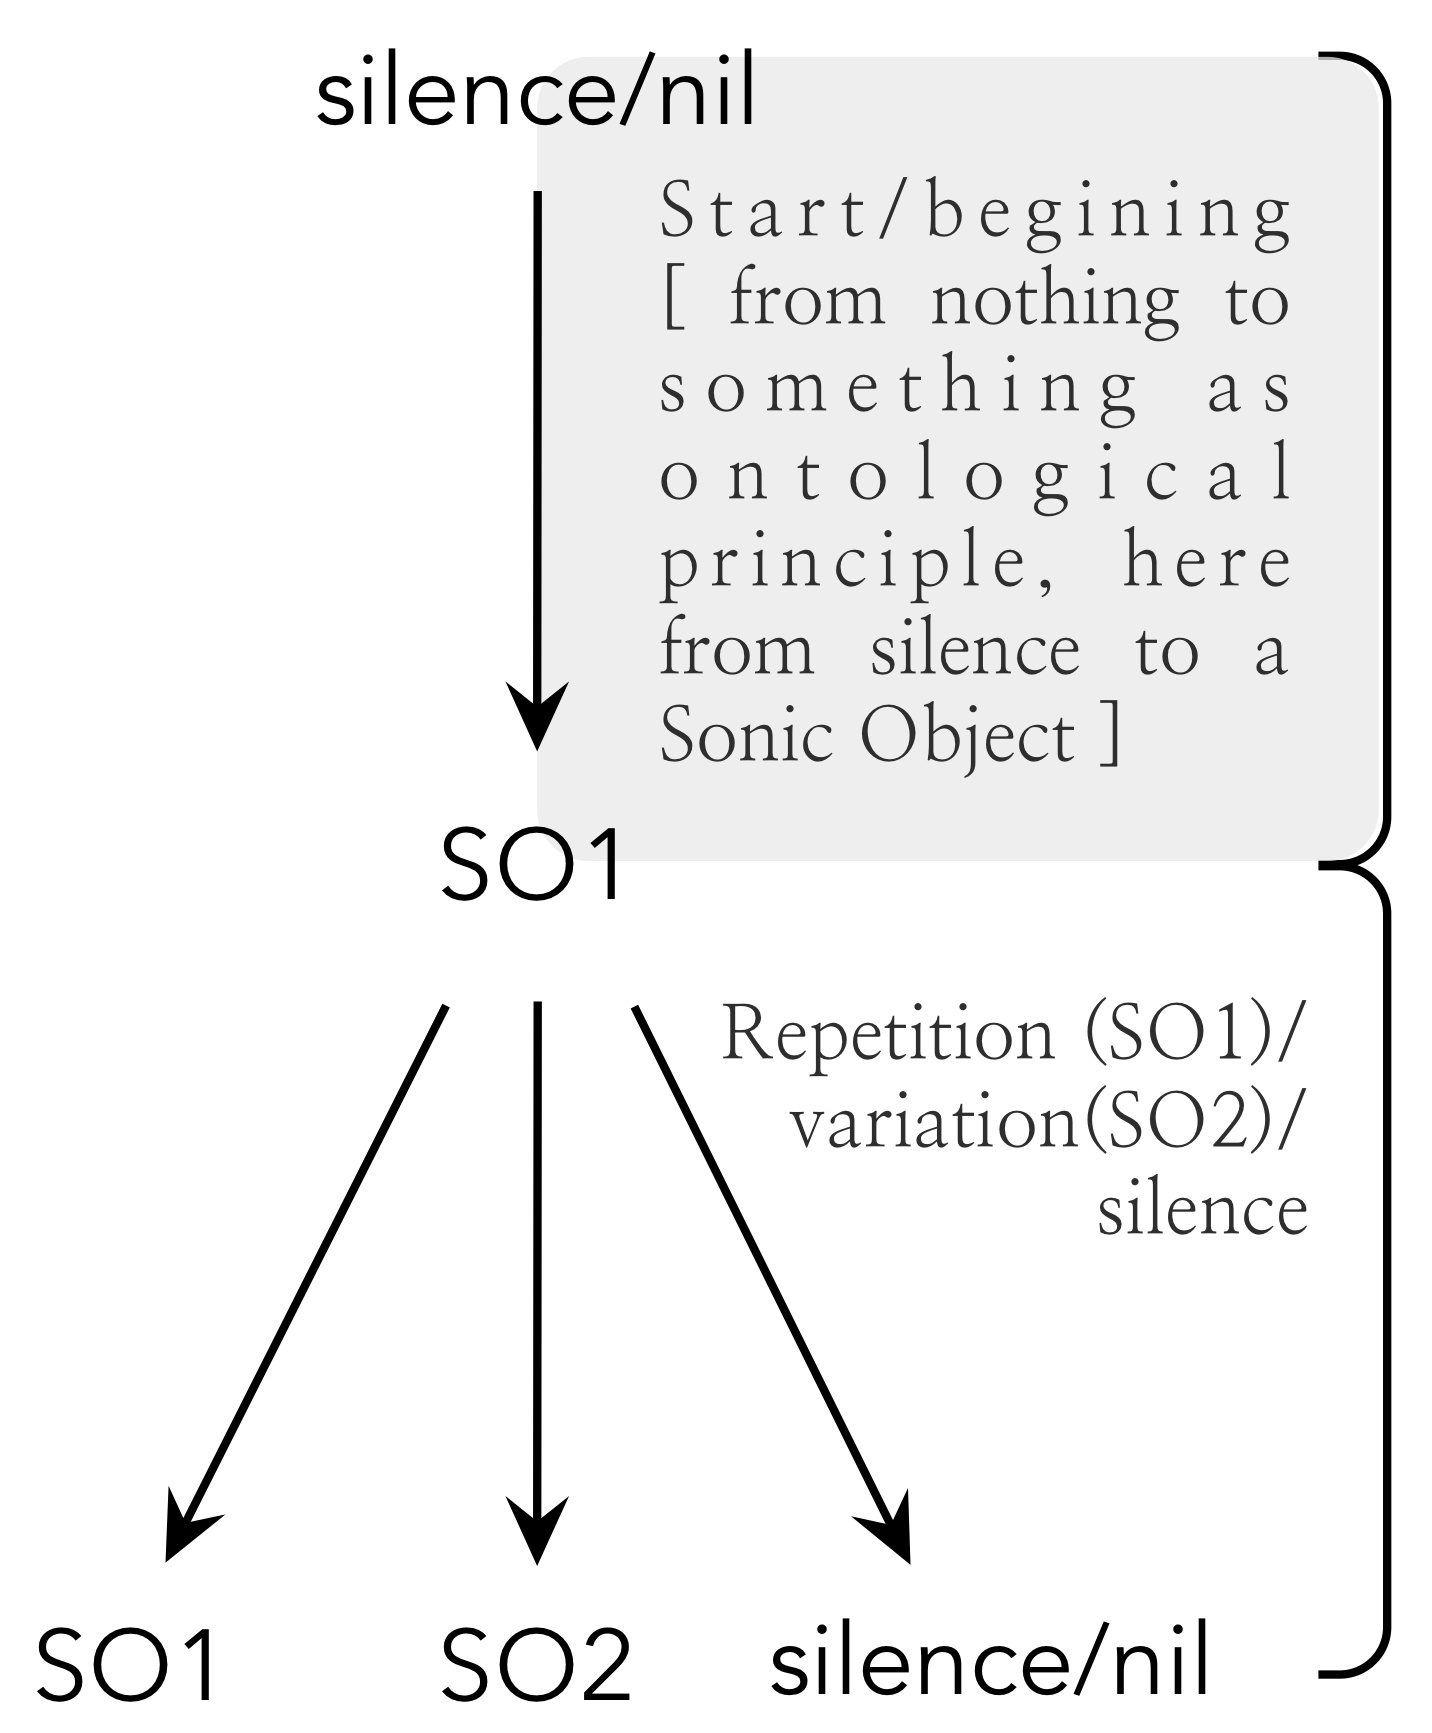
\includegraphics[width=0.35\textwidth]{2345}
  \vspace{-20pt}
\end{wrapfigure}

\bigskip

Then, the idea in the context and in the continuation of \textsl{Neuromuse3}\footnote{\href{https://github.com/yannics/N3D}{\texttt{\scriptsize https://github.com/yannics/N3D}}} is to create a kind of emergent intelligence from the network previously described, composed of cliques and \textit{tournois}, by including additional learning process defined by IDEAL based on the experimentation and on the experience. 

\bigskip

It is opportun to underline the philosophical aspect of this approach in terms of modeling including a causal device as computational cognition.

Thus, each agent develops its own understanding of its environment -- i.e. an ontological conception in epistemological terms.

Also, IDEAL implies non-ontological interactional presuppositions -- the ontological aspect will be defined by the agent as it experiences its interaction with the environment.

\bigskip

With that in mind, the following short description as paragraphs should help the understanding of the different concepts and processes used in this AI context.

\begin{enumerate}[leftmargin=0cm,itemindent=.5cm,labelwidth=\itemindent,labelsep=0cm,align=left]
\item There is \myuline{no a priori knowledge} of the environment. 

\smallskip

`\textit{It allows us to specify inborn behavioral preferences without specifying a predefined goal.}' [$\rightarrow$ \href{https://projet.liris.cnrs.fr/ideal/mooc/lesson.php?n=041}{41. Introduction}, Georgeon, 2014, \textit{loc. cit.} note \ref{noteideal}]

\smallskip

In other words, only primitive interactions -- i.e. innate -- are defined through the initial function, which can evolve over time through the function \texttt{agent-result}. 

\smallskip

`\textit{This design choice follows from constructivist epistemology which suggests that sensorimotor patterns of interaction constitute the basic elements from which the agent constructs knowledge of the world.}' [$\rightarrow$ \href{https://projet.liris.cnrs.fr/ideal/mooc/lesson.php?n=043}{43. Architecture}, Georgeon, 2014, \textit{ibid.}] 

\smallskip

The environment is therefore understood by the AI in terms of reading/writing relevant informations through neurons stimulation device and can be managed by programming constraints.
\end{enumerate}

\bigskip
\bigskip

\noindent {\large \textbf{Glossary}}

\bigskip

Abbreviations: \textsl{fr.} = French; \textsl{acc.} = \textit{acception}.

\begin{description}
\item[Abstract]: is an experiment or a result which refer to an interaction.
\item[Enaction]: interaction with the environment.
\item[Primitive]: low-level interaction defined by the couple experiment/result.\item[Proclivity]: [\textsl{fr}. \textit{propension}] inner, innate, natural force, which directs spontaneously or voluntarily towards an action, a behavior.
\item[Valence]:  [\textsl{acc.} psychology] refers to the intrinsically pleasant or unpleasant quality of a stimulus or situation.
\end{description}

\bigskip
\bigskip

\noindent {\large \textbf{Index}}

\bigskip


\begin{description}[font=\ttfamily]

\item[*PROCLIVITY*] \textit{<t/nil>}

\item[*REMANENCE*] \textit{<integer>}

\item[*VERBOSE*] \textit{<t/nil>}

\item[ADD-OR-GET-EXPERIMENT] \textit{<existence>} \textsl{\&key} label \textit{<symbol>} string \textit{<string>}

\item[ADD-OR-GET-INTERACTION] \textit{<existence>} \textit{<experiment/pre-interaction>} \\ \textit{<result/post-interaction>} \textsl{\&key} valence \textit{<number>} learn \textit{<t/nil>}

\item[ADD-OR-GET-RESULT] \textit{<existence>} \textsl{\&key} label \textit{<symbol>} string \textit{<string>}

\item[CREATE-AGENT] \textit{<name>}

\item[GET-PRIMITIVE-EXPERIENCE] \textit{<experiment/interaction>}

\item[PICK-EXPERIMENT] \textit{<existence>}

\item[PICK-OTHER-EXPERIENCE] \textit{<existence>} \textit{<experiment>}

\item[PREDICT] \textit{<existence>} \textit{<experiment/interaction>} \\ From \textit{existence-interactions}, the evaluation is a \textit{result}.

\item[>REMANENCE] \textit{<existence>} \textit{<experiment/interaction>} \\ Update of \textit{existence-previous} by adding an \textit{experiment} or an \textit{interaction} in the MCT (short-term memory) with |MCT| = \texttt{*REMANENCE*}

\item[RUN-AGENT] <\textit{name}> \textsl{\&key} duration \textit{<integer>} step \textit{<function>} \\ result \textit{<function>}

\item[SELECT-ANTICIPATE] \textit{<existence>} \textit{<experiment/interaction/null>} \\ From \textit{existence-interaction}(s), the evaluation is an \textit{interaction}.

\end{description}

\bigskip
\bigskip

 \begin{notes}

{\large \textbf{Summary description}}

\begin{description}
\item[\texttt{E010}] 
When the expected or desired result is effective, according to the conditions of \texttt{result010}, the qualitative character self-satisfied is `activated' (frustrated otherwise). After $n$ identical, similar, equivalent or other interactions, this is the bored character that is activated, and the system look for another experience to avoid `boredom'.

\item[\texttt{E020}]
The character is quantified with the valence expressing the motivation. This is applied to the primitive interactions.

\quad -- valence $\geq 0 \Rightarrow$ pleased

\quad -- valence $< 0 \Rightarrow$ pained

\item[\texttt{E030}]
Continuation of \texttt{E020} including composite interactions -- i.e. first level abstractions.

\item[\texttt{E031}]
Variation of \texttt{E030} involving weights in terms of proclivity. 

\mynoteuline{The proclivity is estimated as the product of the weight and the} \mynoteuline{valence of the considered interaction.}

\end{description}

\end{notes}





\bigskip
\bigskip

\begin{lstlisting}[language=sectitle]
N3> (format t "~A~&;~v@{~A~:*~}~&" *PART-6* 36 #\*)
SEQUENCING
;************************************
NIL
N3> 
\end{lstlisting}
\addcontentsline{toc}{part}{Sequencing}

\bigskip
\noindent {\large \textbf{Dynamic Markov Chain}}

\bigskip

See  4.7, 5.5.4 and 6.4 in \textsl{Journal of Generative Sonic Art} \citep{yi}. In short, what I call a `Dynamic Markov Chain' allows increasing or coercion decreasing the order in a manner that the transition probabilities do not reach 100\% for a single event.
\bigskip
\bigskip

\begin{lstlisting}[language=sectitle]
N3> (format t "~A~&;~v@{~A~:*~}~2&" *END-PART* 36 #\*)
DOCUMENTATION
;************************************

NIL
N3> (format t "~A" *CHAPTER-A*)
INDEX
NIL
N3> 
\end{lstlisting}
\addcontentsline{toc}{part}{Documentation}
\phantomsection
\addcontentsline{toc}{section}{Index}

\renewcommand*{\glossarypreamble}{\vspace{-1cm}}
\printglossary[title={}] 
\glsaddallunused

\begin{figure}[htbp]
\begin{center}
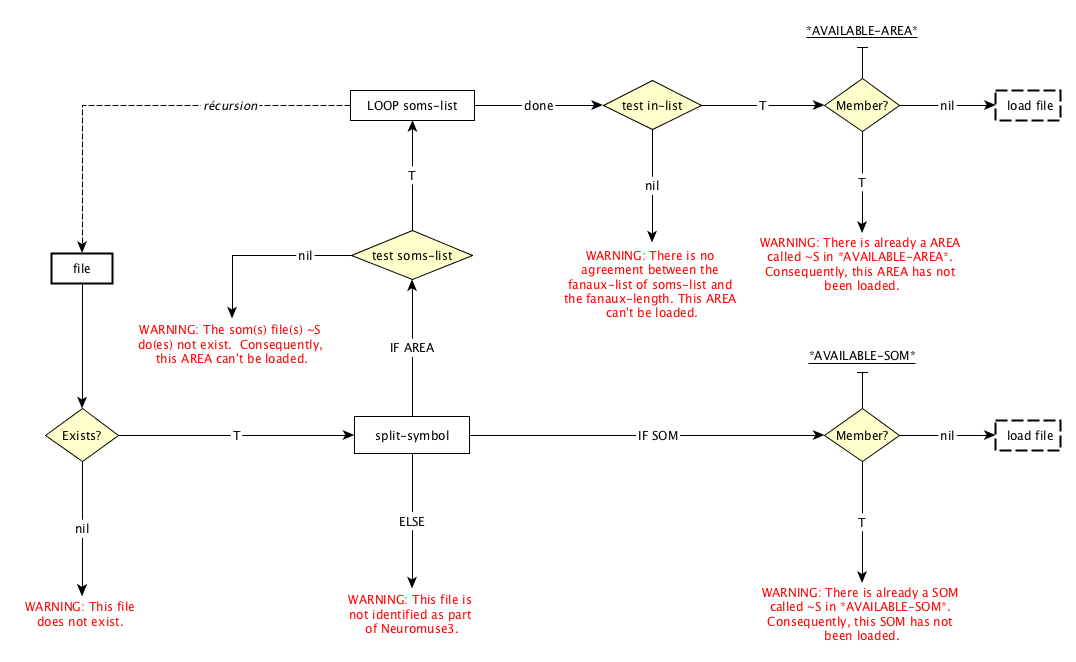
\includegraphics[width=\columnwidth]{2801}
\caption{Synoptic diagram of \glspl{load-neural-network}.}
\label{fig:lnn}
\end{center}
\end{figure}

%\bigskip
%\vspace{-5mm}
\begin{lstlisting}[language=sectitle]
N3> (format t "~A" *CHAPTER-B*)
REFERENCES
NIL
N3> 
\end{lstlisting}
\addcontentsline{toc}{section}{References}
\vspace{-1cm}
\renewcommand{\refname}{}

\renewcommand\bibpreamble{$\rightarrow$ The references to go further or deeper for advanced readers are prepended by an asterisk.\bigskip}

\begin{thebibliography}{99}
		
	\bibitem[Berrou et al., sept 2012]{bg3}
	 * Claude Berrou, Vincent Gripon. \textit{Nearly-optimal associative memories based on distributed constant weight codes}. Information Theory and Applications Workshop, September 2012, pp. 269 to 273.\\ \href{https://www.researchgate.net/publication/254026422\_Nearly-optimal\_associative\_memories\_based\_on\_distributed\_constant\_weight\_codes}{\scriptsize{\texttt{https://www.researchgate.net/publication/254026422}}} \normalsize{}
	
	\bibitem[Berrou et al., 2012]{bg1} 
	Claude Berrou, Vincent Gripon. \textit{Petite mathématique du cerveau -- Une théorie de l’information mentale}. Odile Jacob, 2012.
	
	\bibitem[Berrou et al., 2011]{bg2}
	 * Claude Berrou, Vincent Gripon. \textit{Sparse Neural Networks With Large Learning Diversity}. IEEE transactions on neural networks, Volume 22, 2011, pp. 1087 to 1096.\\ \href{https://arxiv.org/pdf/1102.4240}{\scriptsize{\texttt{https://arxiv.org/pdf/1102.4240}}} \normalsize{}
	 
	 \bibitem[Damasio, 2010]{dam}Antonio Rosa Damasio. \textit{L'erreur de Descartes}. Odile Jacob, Paris 2010.
	 	 
	 \bibitem[Klein, 2020]{cse}
	 CentraleSupélec. \textit{Cours d'Etienne Klein : les deux théories de la relativité d'Albert Einstein}. 
	 YouTube, 23 avril 2020. \\ \href{https://www.youtube.com/watch?v=1NQ6WHDgtM0}{\scriptsize{\texttt{https://www.youtube.com/watch?v=1NQ6WHDgtM0}}} \normalsize{}
	 
	 \bibitem[Chavent, 2013]{mc}
	 Marie Chavent. \textit{La classification automatique de données quantitatives}. 
	 Institut de Mathématiques de Bordeaux UMR 5251, 2013.\\ \href{http://www.math.u-bordeaux.fr/\~mchave100p/wordpress/wp-content/uploads/2013/10/cours\_classif\_quanti.pdf}{\scriptsize{\texttt{http://www.math.u-bordeaux.fr/$\sim$mchave100p/.../2013/10/cours\_classif\_quanti.pdf}}} \normalsize{}
	 
	 \bibitem[Demoures et al., 2005]{fxd}
	 François-Xavier Demoures, Eric Monnet. \textit{Le monde à l’épreuve de l’imagination. Sur << l’expérimentation mentale >>}. Tracés, 2005 \\ \href{https://journals.openedition.org/traces/177}{\scriptsize{\texttt{https://journals.openedition.org/traces/177}}} \normalsize{}
	 
	 \bibitem[Georgeon et al., 2011]{ger}
	 Olivier Georgeon, Frank Ritter. \textit{An intrinsically-motivated schema mechanism to model and simulate emergent cognition}. 
	 Cognitive Systems Research, 2011. {\scriptsize [ doi:10.1016/j.cogsys.2011.07.003 ]}
	 \\ \href{https://projet.liris.cnrs.fr/ideal/doc/GeorgeonO2011-emergent-cognition.pdf}{\scriptsize{\texttt{https://projet.liris.cnrs.fr/ideal/doc/GeorgeonO2011-emergent-cognition.pdf}}} \normalsize{}
	 
	 \bibitem[Goldberg, 2001]{re}
	 * David Goldberg. \textit{What Every Computer Scientist Should Know About Floating-Point Arithmetic}. Numerical Computation Guide, July 2001, pp. 171 to 264.\\ \href{https://ece.uwaterloo.ca/\~dwharder/NumericalAnalysis/02Numerics/Double/paper.pdf}{\scriptsize{\texttt{https://ece.uwaterloo.ca/$\sim$dwharder/NumericalAnalysis/02Numerics/Double/paper.pdf}}} \normalsize{}
	 
	 \bibitem[Ics, 2014/20]{yi}
	 Yann Ics. \textit{Journal of Generative Sonic Art}. Web publication, 2014/2020.\\ \href{https://www.overleaf.com/read/sjhfhthgkgdj}{\scriptsize{\texttt{https://www.overleaf.com/read/sjhfhthgkgdj}}} \normalsize{}
	
	 \bibitem[Jiang et al., 2012]{bg4}
	 * Xiaoran Jiang, Vincent Gripon, Claude Berrou. \textit{Learning long sequences in binary neural networks}. 4th International Conference on Advanced Cognitive Technologies and Applications, July 2012, pp. 165 to 170.\\ \href{https://www.researchgate.net/profile/Xiaoran\_Jiang/publication/265508848\_Learning\_Long\_Sequences\_in\_Binary\_Neural\_Networks/links/54107a6c0cf2f2b29a410d8c.pdf}{\scriptsize{\texttt{https://www.researchgate.net/profile/Xiaoran\_Jiang/publication/265508848}}} \normalsize{}
	 
	 \bibitem[McCarthy, 2007]{jmc}
	 John McCarthy. \textit{From here to human-level AI}. 
	 Artificial Intelligence, Volume 171, Issue 18, 2007, pp. 1174 to 1182. {\scriptsize [ doi:10.1016/j.artint.2007.10.009 ]}
	 \\ \href{https://www.sciencedirect.com/science/article/pii/S0004370207001476}{\scriptsize{\texttt{https://www.sciencedirect.com/science/article/pii/S0004370207001476}}} \normalsize{}
	 
	 \bibitem[McLuhan, 1964]{mm} 
	Marshall McLuhan. \textit{Understanding Media -- The Extensions of  Man}. First edition 1964, MIT Press edition, 1994.
				 
	 \bibitem[Shalizi, 2009]{cs}
	 Cosma Shalizi. \textit{Distances between Clustering, Hierarchical Clustering}. 
	 36-350, Data Mining, 2009.\\ \href{http://www.stat.cmu.edu/\~cshalizi/350/lectures/08/lecture-08.pdf}{\scriptsize{\texttt{http://www.stat.cmu.edu/$\sim$cshalizi/350/lectures/08/lecture-08.pdf}}} \normalsize{}
	 
	  \bibitem[Wells, 1896]{hgw} 
	Herbert-George Wells. \textit{L'Ile du docteur Moreau}. First edition 1896 [\textit{The Island of Dr. Moreau}], Club fran\c{c}ais du livre, Paris 1961. Traduction Henry Durand-Davray. 
		 
\end{thebibliography}
\bigskip
\bigskip

%\newpage
\begin{lstlisting}[language=sectitle]
N3> (format t "~A" *CHAPTER-C*)
BIBLIOGRAPHY
NIL
N3> 
\end{lstlisting}
\addcontentsline{toc}{section}{Bibliography}
\vspace{-1cm}
\renewcommand{\refname}{}
\makeatletter
\renewcommand\@biblabel[1]{}
\makeatother
\renewcommand\bibpreamble{$\rightarrow$ Here is the list of books, articles and  web pages that have been used in some way in the development of this work.\bigskip}

\begin{thebibliography}{99}
        		 
        \bibitem[-, 2012]{}Sous la direction de Daniel Andler. \textit{Introduction aux sciences cognitives}. Gallimard, 2012.
        \bibitem[-, 1995]{}Christophe Assens. \textit{Connexionnisme et théorie des organisations}. Cahiers de Recherche DMSP n°240, Novembre 1995.\\ \href{https://www.christophe-assens.fr/articles/cahier-de-recherche/}{\scriptsize{\texttt{https://www.christophe-assens.fr/articles/cahier-de-recherche/}}} \normalsize{}
        \bibitem[-, 2006]{}Hugues Bersini. \textit{De l'intelligence humaine à l'intelligence artificielle}. Ellipses, Paris 2006.
        \bibitem[-, 2012]{}Ludwig Von Bertalanfy. \textit{Théorie générale des systèmes}. Dunod, Paris 2012.
        \bibitem[-, 2011]{}Pierre Buser, Claude Debru. \textit{Le temps, instant et durée -- de la philosophie aux neurosciences}. Odile Jacob, Paris 2011.
        \bibitem[-, 2005]{}David Michael Cottle. \textit{Computer Music with examples in SuperCollider 3}. Web publication, 2005.\\ \href{http://rhoadley.net/courses/tech\_resources/supercollider/tutorials/cottle/CMSC7105.pdf}{\scriptsize{\texttt{http://rhoadley.net/courses/tech\_resources/supercollider/tutorials/cottle/CMSC7105.pdf}}} \normalsize{}
        \bibitem[-, 2010]{}Antonio Rosa Damasio. \textit{L'erreur de Descartes}. Odile Jacob, Paris 2010.
        \bibitem[-, 2009]{}Colloque annuel 2008 sous la direction de Stanislas Dehaene et Christine Petit. \textit{Parole et musique}. Odile Jacob, Paris 2009.
        \bibitem[-, 2002]{}Jean-Paul Delahaye. \textit{L'intelligence et le calcul -- de Gödel aux ordinateurs quantiques}. Belin, Pour la science 2002.
        \bibitem[-, 1974]{}Jean Fourastié. \textit{Comment mon cerveau s'informe -- Journal d'une recherche}. Robert Laffont, 1974.
                \bibitem[-, 1996]{}Peter Hadreas. \textit{Searle versus Derrida ?}. Philosophiques, Volume 23, n°2, 1996, pp. 317-326. Traduction Josette Lanteigne.\\ \href{https://doi.org/10.7202/027399ar}{\scriptsize{\texttt{https://doi.org/10.7202/027399ar}}} \normalsize{}

        \bibitem[-, 2014]{}Arslan Hamza Cherif. \textit{Neurogrid : un circuit intégré pour simuler 1 million de neurones}. Web publication, 2014.\\ \href{https://www.developpez.com/actu/70629/Neurogrid-un-circuit-integre-pour-simuler-1-million-de-neurones-9-000-fois-mieux-qu-une-simulation-sur-ordinateur/}{\scriptsize{\texttt{https://www.developpez.com/actu/70629/}}} \normalsize{}
        \bibitem[-, 2004]{}Jocelyne Kiss. \textit{Composition musicales et sciences cognitives - Tendances et perspectives}. L'Harmattan, 2004.
        \bibitem[-, 2012]{}Rémy Lestienne. \textit{Dialogues sur l'émergence}. Le Pommier, Paris 2012.
        \bibitem[-, 2011]{}Pierre Mercklé. \textit{Sociologie des réseaux sociaux}. La découverte, Paris 2011.
        \bibitem[-, 2008]{}Alp Mestan. \textit{Introduction aux Réseaux de Neurones Artificiels Feed Forward}. Web publication, 2008.\\ \href{https://alp.developpez.com/tutoriels/intelligence-artificielle/reseaux-de-neurones/}{\scriptsize{\texttt{https://alp.developpez.com/tutoriels/intelligence-artificielle/reseaux-de-neurones/}}} \normalsize{}
        \bibitem[-, 1994]{}Israel Rosenfield. \textit{L'invention de la mémoire}. Flammarion, 1994.
        \bibitem[-, 2011]{}Denis Shasha, Cathy Lazere. \textit{Quand la vie remplace le silicium -- Aux frontières de la bio-informatique}. Dunod, Paris 2011.
        \bibitem[-, 1989]{}Rupert Sheldrake. \textit{La mémoire de l'univers}. Édition du Rocher, 1989.
        \bibitem[-, 2012]{}Rupert Sheldrake. \textit{Réenchanter la science}. Albin Michel, Paris 2012.
        \bibitem[-, 2001]{sn} Bob Snyder, Robert Snyder. \textit{Music and Memory: An Introduction}. A Bradford Book Mit Press, 2001.\\ \href{https://monoskop.org/images/f/f3/Snyder\_Bob\_Music\_and\_Memory\_An\_Introduction.pdf}{\scriptsize{\texttt{https://monoskop.org/images/f/f3/Snyder\_Bob\_Music\_and\_Memory\_An\_Introduction.pdf}}} \normalsize{}
        \bibitem[-, 2014]{}Richard Solé, Bernat Corominas Murtra, Jordi Fortuny. \textit{La structure en réseaux du langage}. Dossier hors-série Pour la science, n°82 janvier/Mars 2014, pp. 8-15.        
        \bibitem[-, 2005]{}Caroline Tourbe. \textit{Nous avons un deuxième cerveau!}. Science \& vie, n°1058 novembre 2005, pp. 64-79.
        \bibitem[-, 2016]{}Andrea Valle. \textit{Introduction to SuperCollider}. The MIT Press, 2016.\\ \href{https://www.scribd.com/document/381922613/intro-to-SuperCollider-pdf}{\scriptsize{\texttt{https://www.scribd.com/document/381922613/intro-to-SuperCollider-pdf}}} \normalsize{}
        \bibitem[-, 2011]{}Scott Wilson, David Cottle, Nick Collins. \textit{The SuperCollider Book}. The MIT Press, 2011.\\ \href{https://www.scribd.com/doc/296526523/The-Supercollider-Book-Scott-Wilson-David-Cottle-Nick-Collins}{\scriptsize{\texttt{https://www.scribd.com/doc/296526523/}}} \normalsize{}
                
        \bibitem[-, 2016]{}Les Dossiers de Sciences \& Univers. \textit{Votre cerveau va vous étonner!}. n°4 novembre 2015/janvier 2016
        
\end{thebibliography}

\bigskip
\bigskip

\begin{lstlisting}[language=sectitle]
N3> (format t "~A~&;~v@{~A~:*~}~&" *NOTE* 36 #\*)
APOSTIL
;************************************
NIL
N3> 
\end{lstlisting}
\addcontentsline{toc}{part}{Apostil}

\bigskip

This documentation aimed to present the \textsl{Neuromuse3} project to this point in time. Also, the project is intended as a reflection about what can be an Artificial Intelligence in a musical context. 

Some work needs to be completed, some other achieved.

\bigskip

The \textsl{Long-term memory} part has to be experimented more deeply, especially for the (re-)construction of sequences. 

\bigskip

The coding of the \textsl{Developmental learning} part is still ongoing. 
After that, one has to merge IDEAL with AREA, by creating classes able to manage both systems. The scope of this work is to say the least about the philosophical approach it is possible to envisage, and on which terms. Indeed, in music, the `walls' are not  fixed and solid objects. The musical environment is very dependant of what has been learned and how forged by its own ontology. Moreover, the character `sensitive' -- which must be linked to a kind of mood -- has to be defined in terms of computing language. The challenge seems daunting, but one must take it up, at least because it can learn a lot about us as a human being.

\bigskip

Thanks for any support or contribution you could bring ...

\bigskip 
\bigskip

%\newpage
\centerline{\texttt{{\footnotesize ... to be continued ...}}}
\begin{figure}[htbp]
\begin{center}

\includegraphics[width=2.7cm]{2223}
\end{center}
\end{figure}
\vspace{-5mm}
\centerline{\texttt{{\footnotesize ... work in progress ...}}}

\end{document}